\chapter{AV1低延迟直播系统构建与优化}

\section{AV1低延迟直播系统构建}

  AV1低延迟直播系统原型如图\ref{fig:av1-sys}构建,主播端摄像头采集图像,进行H.264编码后,通过SRT协议传输到转码服务器,转码服务器使用FFmpeg,调用SVT-AV1编码器将接收到的码流进行H.264到AV1的转码,转码后进行RTP封装后,通过RTSP协议传输到观众端解码播放。

  \begin{figure}[!htp]
    \centering
    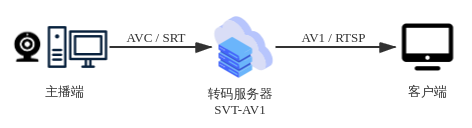
\includegraphics[width=0.6\textwidth]{av1-sys.png}
    \caption{AV1低延迟直播系统原型}
   \label{fig:av1-sys}
  \end{figure}

  % AV1低延迟直播系统原型基于FFmpeg搭建。

\section{AV1低延迟直播系统优化}

\subsection{SVT-AV1的高启动延迟优化}
  搭建的AV1低延迟直播系统原型带有6秒左右SVT-AV1带来的高启动延迟。延迟产生的原因有两个:

  \begin{enumerate} [label=\arabic*)]
    \item \textbf{分配内存多、单线程分配。}SVT-AV1编码器在启动时需要分配大量内存,启动大量线程,本身耗时较长,SVT框架在CPU核心数较多的服务器上会分配更多的线程,而分配线程与内存的工作由单线程完成。这导致在搭载Intel Xeon8280的服务器上,SVT-AV1对于1080p视频参数的启动需要花费6秒进行初始化。
    \item \textbf{编码器启动顺序限制。}AV1直播系统原型中,SVT-AV1编码器作为FFmpeg的plugin被调用,在转码设定下,FFmpeg在服务器端会阻塞式地监听SRT传输端口,需要接收到上行码流,根据解码得到的视频相关参数后才可以进行SVT-AV1编码器初始化。二者的顺序本身不能颠倒,除非事先确定了上行码流的视频分辨率大小。
  \end{enumerate}

  % TODO 格式:enumerate的缩进和后续段落的缩进
  由以上原因,对SVT-AV1的高启动延迟优化有两种方案:

  \paragraph{优化malloc减小初始化延迟} SVT-AV1的debug版本带有对malloc的profile,可以分析初始化过程中,malloc被高频调用的位置。通过对高频malloc的代码进行向量化以大幅减小malloc调用次数,可以一定程度上减小SVT-AV1初始化时间。

  \begin{table}[!hpt]
    \caption{SVT-AV1 malloc优化结果}
    \label{tab:malloc}
    \centering
    \begin{tabular}{ccc} \toprule
      优化    & 初始化时间 & malloc次数\\ \midrule
      优化前  & 6.630s   & 1964126  \\
      优化后  & 5.635s   & 331625   \\ \bottomrule
    \end{tabular}
  \end{table}

  \paragraph{预启动SVT-AV1消除初始化延迟} 上述优化malloc的方法以及其他优化初始化速度的方法只能在一定程度上减小SVT-AV1的初始化时间。对于低延迟的直播系统,要求尽量减小直播系统延迟,可以通过预启动SVT-AV1编码器来消除初始化延迟,这需要约定上行码流的分辨率,因为预启动的行为本身是使用了不能预先获知的信息。在FFmpeg接收到上行码流前按照约定的分辨率预先初始化\texttt{AVCodec},接收到上行码流后用预先初始化好的\texttt{AVCodec},不再重新初始化,即可消除这部分延迟。

\subsection{FFmpeg中AV1的RTP封装实现}
  由于AV1编码的RTP封装协议\cite{RTPPayloadFormat}仍处于草案阶段,以及AV1的RTP封装协议主要用于WebRTC,在FFmpeg中并没有AV1编码的RTP封装支持,因此,为了实现AV1直播系统原型,实现了FFmpeg中AV1的RTP封装实现。

  由于RTP的packet大小限制为1500 bytes,再加上RTP头部的开销,实际payload可用大小小于1500 bytes。对于视频编码,I帧大小往往会超过这个限制,而一些P帧可能远远达不到这个限制,因此需要对OBU进行拆分和聚合,提高RTP封装的传输效率。根据图\ref{fig:av1rtp-aggr}的聚合头部规则对OBU进行拆分与聚合,封装成RTP packet进行传输,解封装时,根据RTP packet中的聚合头部,将packet接封装为OBU,传到解码器进行解码。

  这部分的实现通过在FFmpeg中加入\texttt{rtpenc\_av1.c}、\texttt{rtpdec\_av1.c}来实现对AV1编码的处理。实际实现时,考虑到OBU聚合规则可能引起的延迟,为了达到尽可能低的延迟,仅对超过RTP payload大小的包进行拆分,不进行聚合。

  \begin{figure}[!htp]
    \centering
    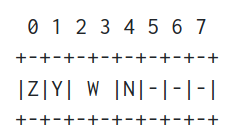
\includegraphics[width=4cm]{av1_rtp_hdr.png} \\
    \raggedright
      \texttt{Z}: 若第一个OBU元素是延续上一个packet的片段,设1,否则设0;\\
      \texttt{Y}: 若最后一个OBU元素是一个会延续到下一个packet的片段,设1,否则设0;\\
      \texttt{W}: 描述当前packet中的OBU元素数量;\\
      \texttt{N}: 若当前packet是视频序列首个packet,设1,否则设0;\\
    \caption{AV1 Aggregation Header}
   \label{fig:av1rtp-aggr}
  \end{figure}

\section{本章小结}
  本章讲述了基于AV1的低延迟编码系统的构建,具体阐述了构建直播系统工作,原型直播系统的构建是后续优化的基础。初始构建的直播系统原型系统延迟较高,将在本章与后续章节中阐述逐步优化的过程。基于所构建的直播系统,在系统层面进行的优化主要有针对SVT-AV1的高启动延迟的优化与实现FFmpeg中AV1的RTP封装。前者通过优化malloc的调用与预启动SVT-AV1编码器解决,后者是在FFmpeg中实现了对AV1码流的RTP封装与解码逻辑。在系统层面进行优化后,由直播系统本身导致的额外延迟基本消除。

%%%%%%%%%%%%%%%%%%%%%%%%%%%%%%%%%%

\chapter{SVT-AV1编码器低延迟优化}

\section{SVT架构}
  Intel的可伸缩视频技术(Scalable Video Technology, SVT)\cite{ScalableVideoTechnology2019}编码器体系结构是专为x86处理器设计的,并且特别针对Intel®Xeon®可扩展处理器进行了大幅优化。SVT架构本身与编码标准无关,它允许将编码器内核拆分为独立运行的线程,每个线程处理视频编码流水线的不同部分。这些线程在不同的处理器内核上并行运行,极大加速了视频编码。SVT-AV1是SVT架构的一个应用实例。

  SVT架构的优势在于其伸缩性,可以根据处理器的核数调整各过程的线程数,因此,对于性能较强的服务器,使用SVT架构可以有效地释放处理器性能,从而提升编码速度;对于性能较差的处理器,SVT架构并不能提升编码速度,反而因为多线程的竞争导致编码速度下降,还因为SVT架构拆分了编码器内核,引入了更多的并行,导致编码效率的下降。对于直播转码服务的场景,往往会使用性能较强的服务器处理,适合SVT架构的发挥。

\subsection{SVT-AV1编码器过程\cite{EncoderDesignSVTAV1}}
  SVT架构是围绕Process过程设计的。过程是软件中的执行线程或硬件中的IP内核。过程执行一个或多个编码器任务(例如,运动估计,速率控制,解块滤波器等)。过程分为基于图像面向控制和面向数据处理两类。控制过程仅允许单个线程实例,因为控制决策必须全局统一,否则有发生数据泄漏和死锁等情况的风险。

  以下简要介绍SVT-AV1中的各个编码器过程:
  \paragraph{资源协调过程(Resource Coordination)} 资源协调进程会收集输入的图像,创建后续编码流水线中会用到的buffer,并将输入的图像与当前的编码器设置一同传递到下一级。

  \paragraph{图像分析过程(Picture Analysis)} 图像分析过程执行编码器预处理分析的第一阶段:图片内图像转换过程,例如重采样,色彩空间转换或色调映射等、创建n-bin直方图以进行场景变化检测,收集图片中每个8x8块的一阶矩和二阶矩统计信息,用于计算方差,输入二次采样和屏幕内容检测。图片分析过程可以是多线程的。

  \paragraph{图像决策过程(Picture Decision)} 图像决策过程执行多图片级别决策,包括设置预测结构,设置图片类型和场景变化检测。由于前一级图片分析过程是多线程的,本级输入可能不按显示顺序到达,因此使用重排序队列来强制按显示顺序对图片进行处理。图像决策过程中使用的算法取决于先前图片的统计信息,因此必须严格保持图片的处理顺序。

  \paragraph{运动估计过程(Motion Estimation)} 运动估计过程使用高度可并行化的,开环的,独立于邻居的方法生成帧间预测和帧内预测候选。运动估计过程中产生的候选成本在下游过程中进一步完善,并且随着更多邻居信息的出现,可以计算出更准确的成本。运动估计由四个部分组成:分层运动估计(HME),搜索中心选择,运动估计和开环内部候选搜索(OIS)。运动估计过程是多线程的,因此只要所有输入都可用,就可以不按顺序处理图片。
  \begin{enumerate} [label=\arabic*)]
    \item HME对下采样的图片执行快速搜索,以收敛到候选搜索中心,以全图片分辨率进行全像素运动估计搜索。
    \item 搜索中心选择使用竞争方法从以下几种方法选择一个搜索中心,包括分层运动估计,时间运动矢量预测值,和外部搜索中心候选。
    \item 运动估计为正在考虑的每个划分在超级块搜索中心附近找到最佳运动矢量。
    \item OIS为每个活动块搜索所有可用的帧内亮度模式,帧内色度模式不考虑。
  \end{enumerate}

  \paragraph{码控初始化过程(Initial Rate Control} 码控初始化过程根据在“图像分析”和“运动估计”过程中收集的数据以及在“图像决策”过程中确定的设置,确定每个图像的初始比特预算。如果允许延迟,则码控初始化过程还将采用滑动窗口缓冲区来分析多张图片。

  \paragraph{基于源的操作过程(Source Based Operation} 基于源的操作过程涉及一些分析算法以识别输入图片的时空特征。一些操作旨在表征单个SB(例如草地区域),一些操作旨在表征整个图片(例如潜在光环区域)。

  \paragraph{图像管理过程(Picture Manager)} 图像管理过程执行管理增强输入图片缓冲区和参考图片缓冲区以及将输入图片细分为图块的功能。增强图片缓冲区和参考图片缓冲区的特定管理都取决于当前使用的GoP结构。图像管理过程使用增强图片和参考图片缓冲区来实现金字塔形B帧GoP结构。图像管理过程以异步操作模式运行,每当接收到增强输入图片或参考图片输入时,就会运行图片管理算法。图片管理算法遍历增强型输入图片缓冲区,并针对每个条目检查参考图片缓冲区中是否有必要的参考图片。如果所有参考都可用,则可以开始图片的编码。

  \paragraph{码控过程(Rate Control)} 码控过程使用在先前过程中生成的失真和图像统计信息,当前图片的比特预算和先前图片统计信息来设置每个图片的QP和比特预算。编码器当前支持VBR类型的码控。

  \paragraph{模式决策配置过程(Mode Decision Configuration)} 模式决策配置过程涉及许多初始化步骤,根据当前的编码器preset,为许多功能设置标志以及确定在后续MD阶段要考虑的模块。

  \paragraph{编码过程(ENCDEC)} 编码过程封装了分块决策阶段,在其中执行许多编码器任务,例如帧内预测,​​运动补偿预测,变换,量化和模式决策。它以运动估计过程的“运动矢量”和失真估计以及码控过程的图片级QP作为输入。编码过程以超级块为单位进行操作。下文会对编码过程有更详细的介绍。

  \paragraph{去块环路滤波过程(Deblocking Loop Filter)} 去块滤波器用于解决重构图片中的块伪像。该过滤器是基于VP9解块过滤器开发的,并在两种类型的过滤器之间切换:窄过滤器和宽过滤器。过滤首先应用于所有垂直边缘,然后再应用于所有水平边缘。

  \paragraph{约束方向增强滤波过程(Constrained Directional Enhancement Filter)} 约束方向增强滤波器(CDEF)在解块滤波器之后应用,旨在改善重构图像。CDEF是Daala编解码器的定向去环滤波器和Thor编解码器的约束低通滤波器(CLPF)的组合,并提供了定向去环滤波和约束低通滤波(CLPF)。

  \paragraph{重建滤波过程(Restortion Filter)} 恢复滤波器是在约束方向增强滤波器之后应用的,其目的是改善重建的图像。涉及两种类型的过滤器:可分离对称维纳滤波器,由于对称性,比特流中仅包含一半滤波器系数;具有子空间投影的自导恢复滤镜,具有保留边缘的平滑效果。

  \paragraph{熵编码过程(Entropy Coding)} 熵编码过程负责为每个帧产生符合AV1的比特流。它以每个块的编码决策和信息为输入,并以每个帧为输出产生比特流。熵编码器是基于帧的过程,并且基于多符号算术范围编码。

  \paragraph{打包过程(Packetization)} 打包过程从每个帧中收集比特流,对时间定界符(TD)以及序列和帧头进行编码,并作为编码器流水线的终点。打包过程将每个帧的比特流以及序列和图片级别的编码设置作为输入,并按图片解码顺序生成最终的比特流。
  \begin{figure}[!htp]
    \centering
    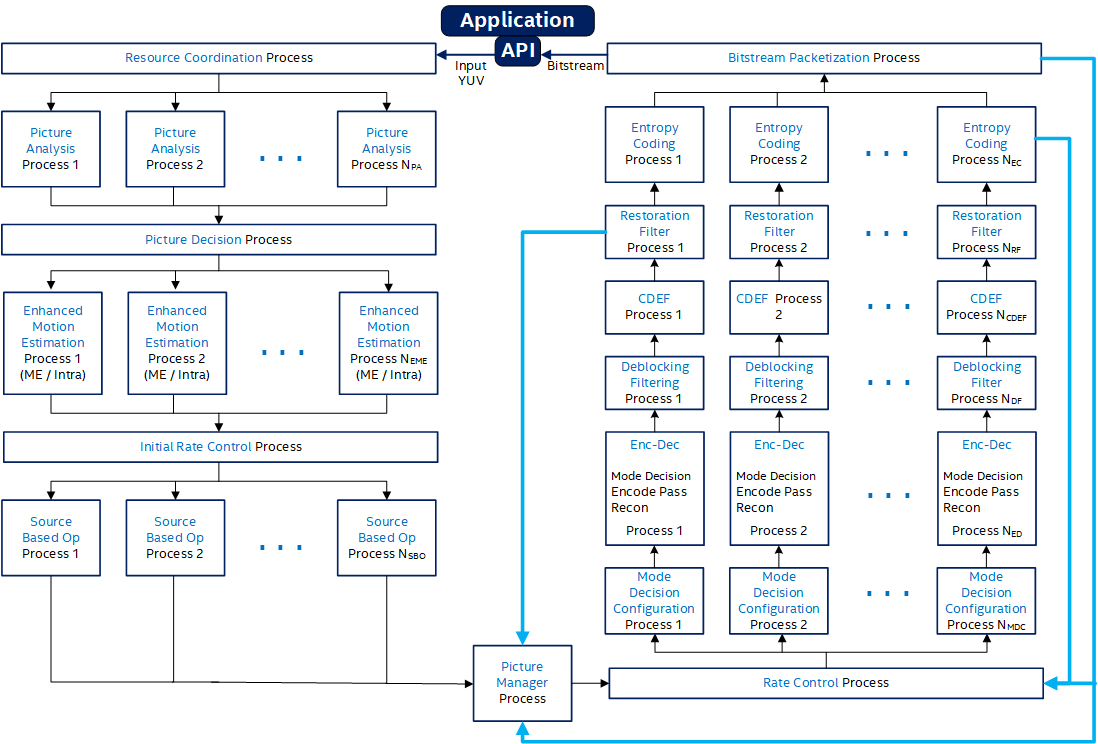
\includegraphics[width=\textwidth]{svt-encoder-process.png}
    \caption{SVT-AV1编码器过程图}
  \label{fig:svt-encoder-process}
  \end{figure}

\subsection{SVT系统资源管理器\cite{EncoderDesignSVTAV1}}

  SVT作为可扩展编码框架的核心是将编码器内核拆分为上述的多个独立运行的过程,这些过程可以根据处理器核心数量实例化为不同数量的线程,SVT系统资源管理器在这其中起到至关重要的作用。系统资源管理器执行过程间数据和控制管理。系统资源管理器通过控制对象的传递方式来管理对象并将不同过程彼此连接,几乎所有过程间通信都通过该链接进行。

  % 这张图很大,要占一页
  \begin{figure}[!htp]
    \centering
    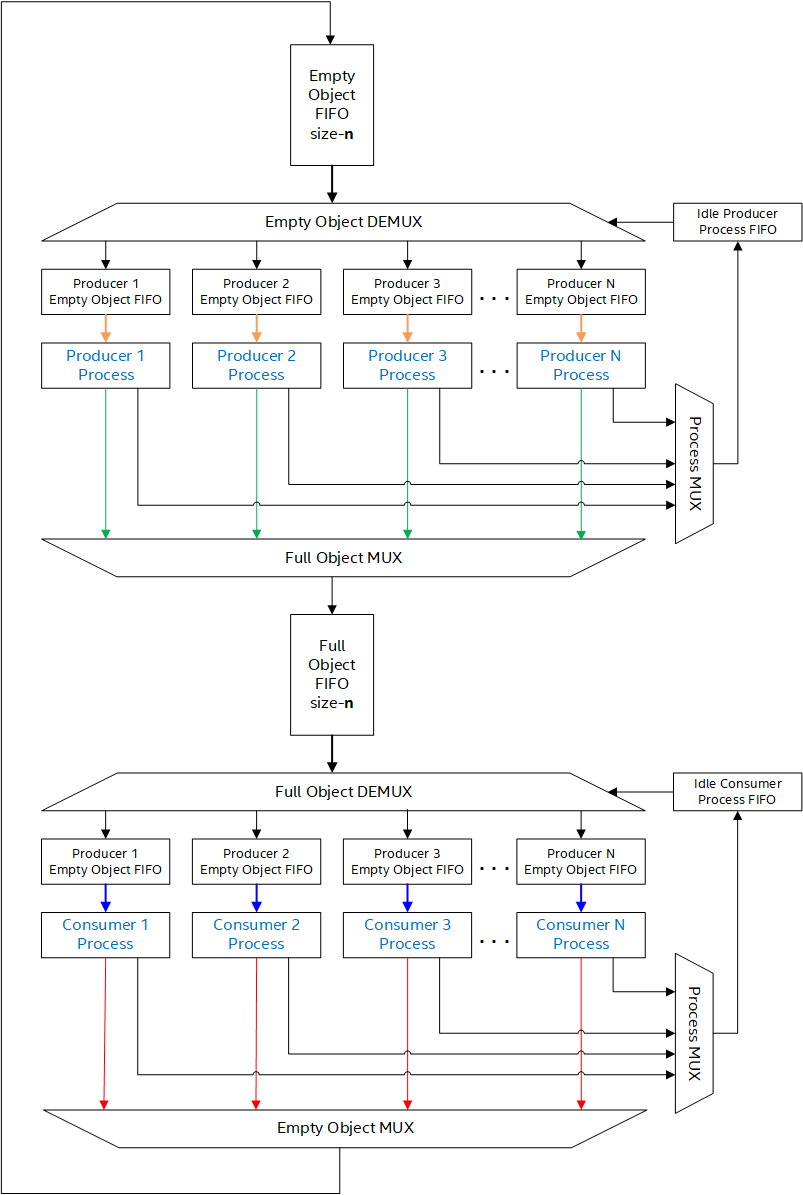
\includegraphics[width=\textwidth]{svt-srm.png}
    \caption{SVT-AV1系统资源管理器示意图}
  \label{fig:svt-srm}
  \end{figure}

  图\ref{fig:svt-srm}展示了系统资源管理器的框图。如图\ref{fig:svt-srm}所示,\texttt{Empty Object DEMUX}将空对象FIFO中的空对象请求\texttt{Process MUX}分配对应的闲置生产者过程,生产者过程用数据和控制信息填充空对象,空对象被填充后成为满对象,被放入满对象FIFO。由\texttt{Full Object DEMUX}为满对象FIFO中的满对象请求\texttt{Process MUX}分配对应的闲置消费者过程。消费者过程使用满对象中的信息进行相应的处理,并通过将现在空对象放回到原始的空对象FIFO中来完成数据流动路径。

  需要注意的是,每个编码器过程既是对象的生产者又是对象的消费者,在当前编码器过程的开始阶段,获取上一级编码器过程生产的满对象,处理后,将结果放入当前编码器过程的空对象,递交到下一级。

  系统资源管理器动态地将对象分配给进程,以最大程度地减少空闲进程时间。另外,空对象路径和完整对象路径的单独协调允许很大的配置灵活性。例如,当生产者和消费者过程需要不同数量的计算资源时,这种灵活性非常重要。在这种情况下,系统资源管理器可能具有N个生产者和M个消费者,其中N不等于M。

  一次典型的编码器内核处理过程如下:
  \begin{enumerate} [label=\arabic*)]
    \item 从上一级内核的\texttt{Full Object DEMUX}获取一个满对象,从中提取待处理的数据或待决策的内容;
    \item 进行当前级编码器内核的处理过程;
    \item 从空对象FIFO中获取一个空对象,将处理结果放入,并将其提交到满对象队列;
    \item 释放起初获取的满对象到空对象队列;
    \item 重复第一步;
  \end{enumerate}

  \subsection{SVT架构的三重并行}
  SVT架构有三重并行:GOP级并行、帧级并行、超级块并行。
  \paragraph{GOP级并行、帧级并行} 当输入的图像帧多于一个GOP大小时,可以同时编码多个GOP。当一个GOP内,帧参考关系满足后,就可以开始对该帧进行编码。具体来讲,在SVT架构中,图像管理过程(PM)之前的过程属于编码前过程,读入图像帧后即可运行,之后的过程开始正式编码,需要参考GOP结构中的其他帧,当参考关系满足后才可以继续。
  \paragraph{超级块并行} 在编码过程(ENCDEC)中,以超级块为单位,波浪形的方式并行处理。由于每个超级块的编码依赖于其左边和上边块,因此,当一个超级块的左边块和上边块完成编码后,该超级块可进入编码。

  \subsection{SVT架构的多阶段分区、模式选择决策\cite{EncoderDesignSVTAV1}} \label{sec:pd-md}
  给定一个超级块可以考虑的大量块划分方式和大量预测模式,使用所有可用编码工具评估所有选项来收敛到最优分块和编码模式在计算上将非常昂贵。因此,SVT架构使用分阶段决策的方法,有分阶段分区决策(Partition Decisions, PD)和分阶段模式选择(Mode Decisions, MD)。

  如图\ref{fig:pd}所示,向PD阶段0输入运动估计结果以及所有可能的分区情况$N_0$,使用比较基本的工具和指标来初步评估不同候选的适应性,并将其中最优的$N_1$种候选传递到PD阶段1,并在后续PD阶段中考虑更复杂的预测和指标来评估。多阶段PD决策后渠道最优的分区决策和模式选择。

  \begin{table}[!hpt]
    \renewcommand{\arraystretch}{0.8}
    \caption{MD阶段处理的9类编码工具候选}
    \label{tab:av1-classes}
    \centering
    \begin{tabular}{cc} \toprule
      序号    & 工具 \\ \midrule
      0& Intra \\
      1& Inter (NEWMV) \\
      2& MV Pred  \\
      3& Inter-Inter compound \\
      4& Intra-Inter compound \\
      5& OBMC \\
      6& Filter Intra \\
      7& Palette prediction \\
      8& Global Motion candidates \\\bottomrule
    \end{tabular}
  \end{table}

  如图\ref{fig:md}所示,在每个PD阶段中,包含多个模式选择MD阶段。PD阶段输入的候选分为9个类别,如表\ref{tab:av1-classes}分别对应AV1的不同编码工具。引入候选类别的主要思想是确保重要类型的候选有机会出现在最后的MD阶段,并在该阶段与其他候选类别的最佳候选竞争。在每个MD阶段中使用预测工具与性能指标评估各个候选,对候选进行筛选,只有性能最好的一部分候选被传递到下一个MD阶段,越靠后的MD阶段中,更多更细致的预测工具与性能指标会被使用。



  \begin{figure}[!htp]
    \centering
    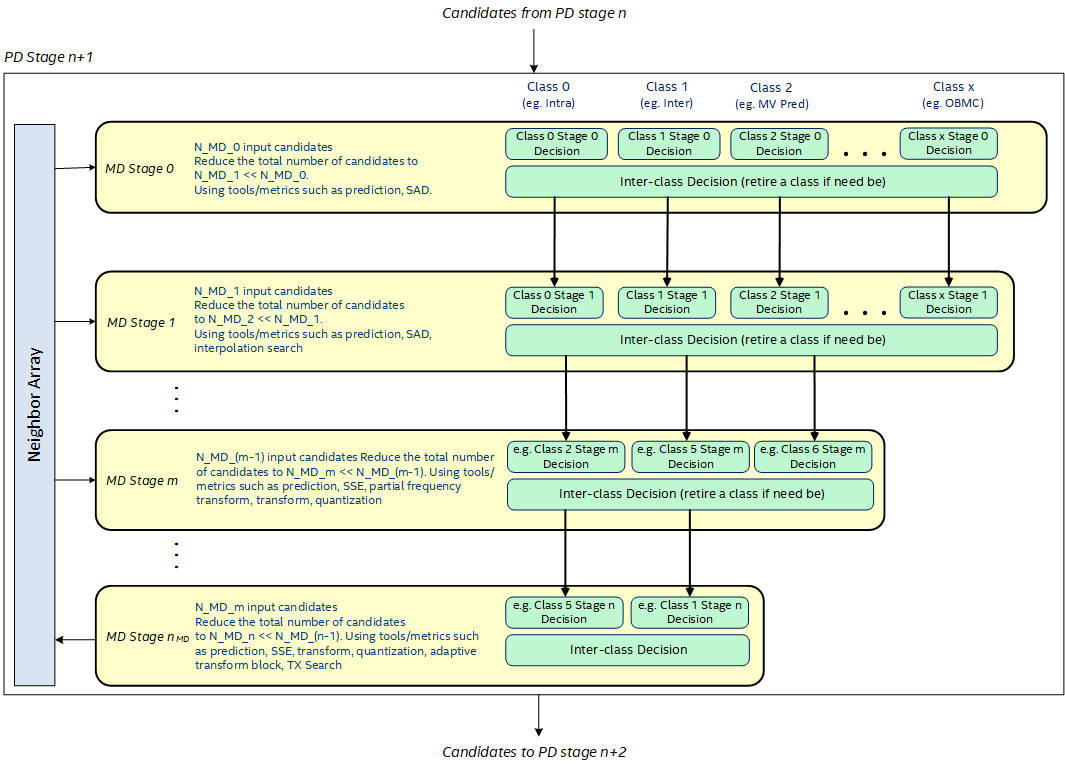
\includegraphics[width=\textwidth]{pd-stages.png}
    \caption{分阶段分区决策\cite{EncoderDesignSVTAV1}}
  \label{fig:pd}
  \end{figure}

  \begin{figure}[!htp]
    \centering
    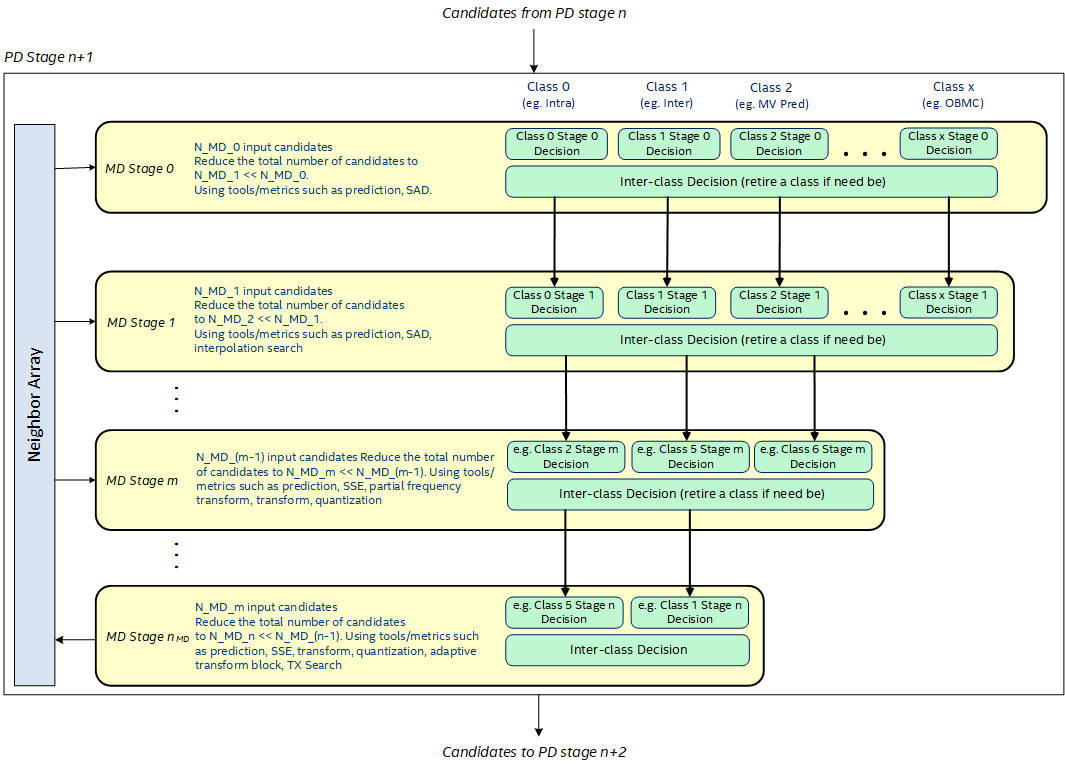
\includegraphics[width=0.7\textwidth]{md-stages.png}
    \caption{单次分区决策中的多阶段模式选择\cite{EncoderDesignSVTAV1}}
  \label{fig:md}
  \end{figure}
  %TODO 写一下AssignSegment的伪代码?
\section{SVT架构的编码延迟profile工具} \label{sec:svt-profile}
  为了分析SVT架构的编码延迟来源,我们需要一个工具帮助我们分析SVT架构内部的延迟。具体有以下要求:
  \begin{enumerate} [label=\arabic*)]
    \item 避免profile工具对SVT-AV1本身的编码速度造成影响。
    \item 可以尽量详细地记录各线程开始、完成每项任务的时间节点。
  \end{enumerate}

  由此设计了SVT的延迟profile工具。因为直接进行文件写入或输出到stdout会对程序运行速度影响较大,选择先写入内存,当编码结束后,统一写入文件,通过这种方式尽量减小对SVT本身编码速度的影响。在每次系统资源管理器进行对象获取或提交时,记录一条带有时间、过程以及处理图像或片段信息的entry。

  表\ref{tab:svt-profile}是编码一帧1080p分辨率的视频帧的延迟测量结果,为了便于展示,表格中省略了一些内容。通过分析延迟测量的结果可以了解SVT架构下各过程的运行情况,便于分析延迟的产生以及产生对应的优化方案。
  % TODO table: latency-profile + table: latency-profile analysis

  \begin{table}[!hpt]
    \renewcommand{\arraystretch}{0.8} % 减小行间距
    \caption{SVT-AV1处理一帧时各过程延迟Profile}
    \label{tab:svt-profile}
    \centering
    \begin{tabular}{ccccccccc} \toprule
      process & inType & outType & picNum & segIdx & tileIdx & sTime & eTime & duration\\ \midrule
      RESOURCE & 0 & 0 & 0 & -1 & -1 & 0.00 & 0.02 & 0.02 \\
      PA & 0 & 0 & 0 & -1 & -1 & 0.10 & 5.84 & 5.74 \\
      PD & 0 & 0 & 0 & 0 & -1 & 5.93 & 5.95 & 0.02 \\
      PD & 0 & 0 & 0 & 59 & -1 & 5.93 & 6.41 & 0.48 \\
      ME & 0 & 0 & 0 & 0 & -1 & 6.04 & 6.05 & 0.01 \\
      ME & 0 & 0 & 0 & 59 & -1 & 6.42 & 6.43 & 0.00 \\
      IRC & 0 & 0 & 0 & -1 & -1 & 6.46 & 6.47 & 0.01 \\
      SRC & 0 & 1 & 0 & -1 & -1 & 6.55 & 6.57 & 0.02 \\
      PM & 1 & 0 & 0 & -1 & -1 & 6.66 & 6.75 & 0.09 \\
      RC & 0 & 0 & 0 & -1 & -1 & 6.79 & 8.28 & 1.49 \\
      MDC & 0 & 0 & 0 & -1 & 0 & 8.36 & 14.86 & 6.50 \\
      ENCDEC & -1 & -1 & 0 & 0 & -1 & 14.94 & 17.25 & 2.31 \\
      ENCDEC & -1 & -1 & 0 & 510 & -1 & 269.88 & 272.44 & 2.56 \\
      DLF & 0 & 0 & 0 & 0 & -1 & 272.51 & 272.51 & 0.01 \\
      DLF & 0 & 0 & 0 & 59 & -1 & 272.51 & 272.98 & 0.47 \\
      CDEF & 0 & 0 & 0 & 0 & -1 & 272.90 & 353.18 & 80.28 \\
      REST & 0 & 0 & 0 & -1 & 0 & 353.29 & 353.86 & 0.57 \\
      ENTROPY & 0 & 2 & 0 & 0 & 0 & 353.87 & 357.16 & 3.29 \\
      ENTROPY & 0 & 2 & 0 & 16 & 0 & 396.35 & 397.56 & 1.21 \\
      PAK & 0 & 0 & 0 & -1 & -1 & 397.80 & 398.13 & 0.32\\ \bottomrule
    \end{tabular}
  \end{table}

\section{SVT架构的延迟优化}
\subsection{RESOURCE过程的EOS优化}
  SVT-AV1本身不是为了低延迟而设计,因此在一些细节需要进一步优化,例如RESOURCE过程中,需要在收到下一帧的输入后才会将当前帧发送给下一级PA过程。这种延后一帧输出的机制是因为流结束标志EOS(End of Stream)设置需要,EOS标记用于表示当前帧是输入流的最后一帧。编码器在发送完最后一帧的数据后,会再发送一个带有EOS标记的空包,指示编码器终止编码过程。

  这样设计的机制在普通视频流编码中是合理的。但是对于我们要求的低延迟编码,EOS机制意味着额外的一个帧输入间隔延迟,对于30fps的流,这个延迟为33ms,相对较大,因此我们可以假设输入的视频流的总帧数是未知的,RESOURCE过程在收到一帧图像后立刻发送给下一级的PA过程,在流需要停止的时候才发送EOS包。
\subsection{分tile优化}
  处于性能考虑,SVT-AV1的分tile机制限制在只能分行,不能分列。这导致编码过程中,每个tile编码的波形并行的tile宽度没有发生变化,在一行上的传播次数不变,使得分tile的编码延迟增益十分有限。为了达到更低的编码延迟,这里选择牺牲一部分编码效率来提高并行率,降低编码延迟。


\section{基于JND的快速编码优化}

  % 能和学长的论文在介绍部分有多少相似性?会查重否?
  \subsection{人眼视觉感知特性} \label{sec:HVS}
  人眼的生理学构造决定了它独特的视觉感知特性。通过研究人眼视觉感知特性,我们可以将人眼视觉系统的主观感受与接收的客观信息建立联系,并将二者的关系数学建模分析。多年的发展以来,已经有一些人眼视觉感知特性被开发,并且对应有较为成熟的理论解释。下面将介绍部分视觉感知特性:亮度特性、视觉掩蔽效应、视觉注意机制等。

  \begin{figure}[!htp]
    \centering
    
\includegraphics[width=0.8\textwidth]{brightness.png}
    \caption{亮度自适应特性}
  \label{fig:brightness}
  \end{figure}

  \paragraph{亮度自适应特性} 亮度自适应特性指的是,当受到多种不同强度的光照下,人眼视觉系统可以通过调节自身对于光强的敏感度来适应较大的亮度范围。通过亮度特性人眼可以调节出的对高达百倍的亮度差的适应性,具体体现在三个方面:对暗部的适性应、对亮部的适应性和局部亮度适应性。由于亮度自适应特性,人类视觉系统对绝对亮度不敏感,对相对亮度敏感,这被称为亮度对比度敏感特性:能够通过视觉目标和背景亮度差值调整自身的亮度感知能力。如图\ref{fig:brightness},五个圆形图案的亮度相同,但随着圆形外部正方形背景亮度的不断降低,人眼感知结果是圆形图案的亮度从左到右逐渐升高。

  % \begin{figure}[!htp]
  %   \centering
  %   
\includegraphics[width=0.8\textwidth]{mach-effect.png}
  %   \caption{马赫效应}
  % \label{fig:mach}
  % \end{figure}

  % 人眼视觉对图像边缘处的增强感受。它指的是当目标物体亮度发生突变,人眼会感觉物体亮度较高的一侧更亮,亮度较暗的一侧会更暗。这种现象导致在发生变化的边缘处人眼会感觉到出现了一条分割线,但是实际上从客观数值上是检测不到这条分割线的。如图\ref{fig:mach}所示,为马赫效应的示意图,其中每个灰度带都相差一个固定的灰度值,人眼在对每两个相邻的灰度带进行观测时,会感觉中间有一条分割线对其进行分割。该效应反映了人类视觉系统的对比增强特性,能够增强目标轮廓,有利于人眼检测出视觉信息上的特定目标。这种特性显示出人类视觉系统会自动增强亮度变化较大的物体的边缘信息,所以在对视觉感知算法进行研究时需要特地考虑边缘的信息。

  \paragraph{视觉掩蔽效应} 视觉掩蔽效应指人类视觉系统在处理多个视觉信号时,由于各视觉信号相互干扰而无法处理全部信号的信息的现象。其具体表现为当目标信号与掩蔽信号同时存在时,导致目标信号被掩蔽信号影响,使其难以察觉。例如在图像压缩中,一些失真出现在特定区域中时不易被察觉,但出现在某些区域时会变得非常明显。研究发现有许多影响掩蔽效应的因素,其中包括视觉信号频率、运动幅度、色度、亮度、纹理复杂度等。常见的视觉掩蔽效应有:运动掩蔽效应、对比掩蔽效应、纹理掩蔽效应等。以下简要介绍三种常见的视觉掩蔽效应。
  \begin{description}
    \item [1) 运动掩蔽效应]
    运动掩蔽效应指的是当目标范围物体运动幅度较大时或相邻视频帧变化较大时,人类视觉系统对这些运动较大的区域敏感度较低,对于其中的细节感知能力较差,难以察觉到这些区域的失真。相对运动幅度较低的区域,运动幅度较大的区域能够容纳更高的图像失真。
    \item [2) 对比度掩蔽效应]
    对比度掩盖效果是指人类视觉系统在比较不同灰度级别的区域的时候产生的掩蔽效果。人眼会根据图像亮度的变化而改变其对各个区域的敏感度,这种影响通常发生在图像的边缘区域。
    \item [3) 纹理掩蔽效应]
    人类视觉系统对纹理复杂度较高区域中的失真不敏感。对于视觉中不同纹理复杂度的内容,人眼纹理复杂度较高的区域出现的失真相比纹理复杂度较低的区域的失真更难被人类视觉系统所察觉,
  \end{description}

  \paragraph{视觉注意机制} 当人类视觉系统处理视觉信号时,并不会对所有视觉信号均给予相同的注意力,而是会将注意力快速切换到更感兴趣的目标物体,对其它不感兴趣的物体则给予较低的关注,这类主动提取感兴趣区域的机制被称作视觉注意机制\cite{borjiStateoftheArtVisualAttention2013}。存在两种提取视觉注意力区域的模式,一种是自上而下,由人类主观意志驱动将注意力集中到某特定区域;另一种是自下而上,在图像区域的显著性影响下,自然地将注意力集中到显著性较强的区域,是被动的过程。两个视觉注意区域模型相互影响,共同完成图像信息的提取与分析处理。因为自上而下的模型会根据不同的处理需求将注意力分配到不同区域,是不确定的,因此当前的算法一般研究自底向上的模式,通过分析基本的图像特性来寻找图像中的显著区域。

  人类视觉系统会将较多的注意力分配到视觉注意机制确定的显著区域,与非显著区域对比,显著区域对图像的质量在视觉上有更大的影响。因此,区分是否显著区域并分别处理可以提高图像主观视觉质量。已有许多基于视觉注意机制的研究应用在视频编码领域,Bai等人提出的基于视觉感兴趣区域(Region of Interest, ROI)的码率控制方案\cite{baiSaliencyBasedRate2016},通过将码率预算优先分配到视觉感兴趣区域从而提高编码性能。

  \subsection{像素级JND模型介绍}
  传统的视频编码旨在去除视频在时域与空域的信息冗余,不考虑对人眼视觉特性的适应性。因此,编码后的视频仍包含许多人眼视觉无法察觉到的冗余,这些感知冗余是我们的优化方向。为了定量处理这些感知冗余,在感知编码中恰可察觉失真(Just-Noticeable-Distortion, JND)模型是一类较好的选择,JND模型根据人眼视觉特性提出,定量描述了人眼恰可察觉的失真阈值,用于度量视频编码中的感知冗余。

  近年来,对JND模型的研究可分为两类:一类是子带域(Subband-domain)JND模型,该类模型在子带域分析,使用该类模型时,需要先将原视频变换到子带域,另一类是像素域JND模型,该类模型直接在原始视频的图像像素域上计算。由于子带域JND模型需要进行频域转换,需要额外的复杂度,在实际应用中效率较低,相对而言,像素域JND由于计算更快,在视频、图像处理中更常用。现有的像素域JND模型一般由亮度适应性和空间对比度掩蔽两部分组成。

  \begin{figure}[!htp]
		\centering
		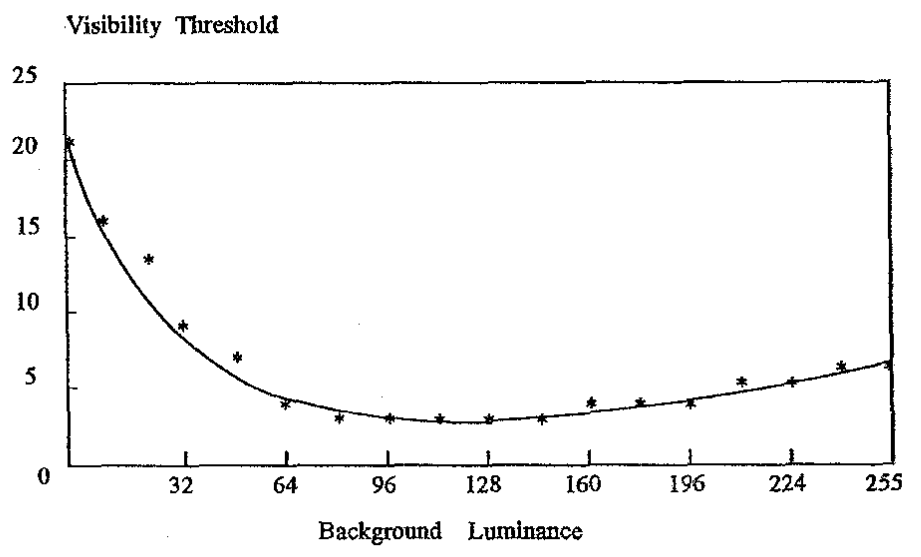
\includegraphics[width=0.66\textwidth]{bg-luma.png}
		\caption{视觉阈值与背景亮度相关曲线\cite{chun-hsienchouPerceptuallyTunedSubband1995}}
		\label{fig:bg-luma}
	\end{figure}
  \paragraph{亮度适应性} 如\ref{sec:HVS}小节,人类视觉系统会根据背景亮度的大小不一表现出不同的视觉敏感度,称为亮度自适应特性(Luminance Adaptation, LA)。文献\cite{chun-hsienchouPerceptuallyTunedSubband1995}表明,人眼的视觉阈值与背景亮度呈非线性关系,其关系如图\ref{fig:bg-luma}所示,当背景亮度低于127时,视觉可见性阈值以幂函数形式下降,当背景亮度高于127时,视觉可见性阈值随背景亮度的增加线性增长。据此,将亮度适应性与视觉阈值的关系建模为基于背景亮度的分段函数\cite{chun-hsienchouPerceptuallyTunedSubband1995},如式\ref{equ:la}所示:

  \begin{equation} \label{equ:la}
    LA(i, j) = \begin{cases}
      \left(1 - \sqrt{\frac{B(i, j)}{127}}\right) \cdot 17, & \mathrm{if}\: B(i, j)\leq 127 \\
      \left(B(i, j) - 127\right) \cdot \frac{3}{128} + 3, &\mathrm{else},
    \end{cases}
  \end{equation}
  其中,$B(i, j)$为图像中像素点$(i, j)$周围$5\times 5$范围内的亮度与图\ref{fig:5x5luma-kernel}所示的卷积核相关结果。

  \begin{figure}
    \hspace{1cm}
		\subcaptionbox{$5\times 5$背景亮度卷积核\label{fig:5x5luma-kernel}}[0.3\textwidth]{
			\begin{tabular}{|c|c|c|c|c|}	\hline
				1 & 1 & 1 & 1 & 1 \\ \hline
				1 & 2 & 2 & 2 & 1 \\ \hline
				1 & 2 & 0 & 2 & 1 \\ \hline
				1 & 2 & 2 & 2 & 1 \\ \hline
				1 & 1 & 1 & 1 & 1 \\ \hline
			\end{tabular}
    }
    \hspace{2cm}
    \subcaptionbox{$8\times 8$背景亮度卷积核\label{fig:8x8luma-kernel}}[0.3\textwidth]{
			\begin{tabular}{|c|c|c|c|c|c|c|c|}	\hline
				1& 2& 2& 3& 3& 2& 2& 1 \\ \hline
				1& 2& 0& 3& 3& 0& 2& 1 \\ \hline
				1& 3& 3& 5& 5& 3& 3& 1 \\ \hline
				1& 3& 3& 5& 5& 3& 3& 1 \\ \hline
				1& 2& 0& 3& 3& 0& 2& 1 \\ \hline
				1& 2& 2& 3& 3& 2& 2& 1 \\ \hline
				1& 1& 1& 2& 2& 1& 1& 1 \\ \hline
			\end{tabular}
		}
    \caption{背景亮度卷积核}
	\end{figure}

  \paragraph{对比度掩蔽效应} 对比度掩蔽效应是一种常见且重要掩蔽效应,指在观看对比度不同的区域时产生的掩蔽效应,相比低对比度的区域,高对比度的区域具有更强的视觉掩蔽效应。根据文献\cite{wuPatternMaskingEstimation2013},对比度掩蔽效应(Constast Masking, CM)可以建模关于亮度对比度的非线性函数,由此得到对比度掩蔽效应因子$CM$,如式\ref{equ:cm}所示:

  \begin{equation} \label{equ:cm}
    CM(i, j) = 0.115 \cdot \frac{\alpha \cdot L_c(i, j)^{2.4}}{L_c(i, j)^2 + \beta^2}
  \end{equation}
  其中$\alpha$和$\beta$为常数,分别取16和26。$L_c(i, j)$为图像中像素点$(i, j)$位置的$5\times 5$范围亮度标准差。
  % question: CM到底如Matlab中的是亮度方差(标准差)还是如黄yc的论文里面写的用梯度、Prewitt算子算的。

  \paragraph{非线性组合模型} 计算得到亮度适应性因子$LA$和对比度掩蔽效应因子$CM$这两种视觉特性强度后,如何有效将它们集成在一起获得准确的JND阈值成为了一个重要问题。考虑到与只存在一种掩蔽效应相比,多个掩蔽效应会导致目标区域的失真更难以察觉,因此多个掩蔽效应的组合应采取某种形式的加法,一方面,两个掩蔽因子之间重叠会导致各自的增益降低,另一方面,需要考虑两个因子之间相互重叠的影响范围。基于以上的考虑,文献\cite{yangJustNoticeableDistortion2005}提出了一种非线性组合模型,能够将两种视觉特性强度进行组合,得到最终的JND感知阈值模型。因此,采用该非线性组合模型对亮度适应性因子$LA$和对比度掩蔽效应因子$CM$组合,得到的JND感知阈值模型,如式\ref{equ:jnd}:

  \begin{equation} \label{equ:jnd}
    \mathrm{JND}(i, j) = LA(i, j) + CM(i, j) - 0.3 \cdot \min \left\{LA(i, j) , CM(i, j)\right\}
  \end{equation}



	\subsection{块级JND模型\label{sec:blk-based-jnd}}
	原始的JND感知阈值模型是像素级模型,处理一个视频帧时,需要对其中的每个像素位置进行计算,运算量较大,严重影响算法的延迟,为了将JND感知阈值模型用在实时的低延迟编码中,需要对模型进行简化。结合后续将JND感知阈值用于分区决策中提前终止算法,将原始的像素级JND感知阈值模型简化为$8\times 8$块级模型,最小处理单位化为$8\times 8$块。式\ref{equ:la}中的亮度均值计算使用的卷积核替换为图\ref{fig:8x8luma-kernel}所示的$8\times 8$卷集合,式\ref{equ:cm}中使用的亮度标准差替换为$8\times 8$块内的亮度标准差。由此计算块级的JND感知阈值$\mathrm{JND_{8x8}}(i, j)$。

	\begin{equation} \label{equ:jnd2}
		\mathrm{JND_{8x8}}(m, n) = LA(m, n) + CM(m, n) - 0.3 \cdot \min \left\{LA(m, n) , CM(m, n)\right\}
	\end{equation}
	其中,$m, n$分别表示视频帧的$8\times 8$块行、列索引。

  根据式\ref{equ:jnd2},可以计算得到视频帧的块级JND感知阈值矩阵。其中的JND感知阈值越高,表示该$8\times 8$块的纹理细节丰富,元素排列无序,掩蔽效应较强,人类视觉系统对其失真的敏感度较低。反之,若JND感知阈值越小,表示该$8\times 8$块较为平坦,元素趋于同质,掩蔽效应较弱,人类视觉系统对失真的敏感度较高。综上,可以根据计算得到的JND感知阈值对视频帧的纹理复杂度与图像失真敏感度进行评估。

  \subsection{基于JND的超级块快速划分优化算法}
  根据文献\cite{guoqingxiangImprovedAdaptiveQuantization2017},计算图像块的JND感知阈值方差可以反映图像块中的感知纹理一致性。若图像块的JND感知阈值方差较大,表示该块中纹理复杂度较高;反之,若图像块的JND感知阈值方差较小,表示该块相对平坦,纹理复杂度较低。在AV1视频编码中,超级块中的图像内容特性决定了超级块划分,一般对于纹理复杂度较高的区域,超级块划分较深,对于平坦的图像内容,超级块划分深度较浅、甚至不划分。图\ref{fig:jnd-sb}展示了一些超级块的划分结果,从左往右,超级块中纹理复杂度逐渐增加,对应的超级块划分更加深入仔细。

  \begin{figure}[!hbtp]
    \centering
    \subcaptionbox{简单纹理}
                    [0.24\textwidth]{
\includegraphics[height=2.5cm]{part_64x64_1.png}\label{fig:jnd-sb-1}}
    % \hspace{1cm}
    \subcaptionbox{稍复杂纹理}%
                    [0.24\textwidth]{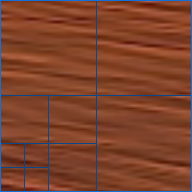
\includegraphics[height=2.5cm]{part_64x64_2.png}}
    \subcaptionbox{更复杂纹理}%
                    [0.24\textwidth]{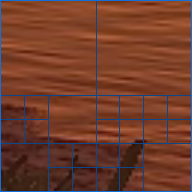
\includegraphics[height=2.5cm]{part_64x64_3.png}}
    % \hspace{1cm}
    \subcaptionbox{复杂纹理}
                    [0.24\textwidth]{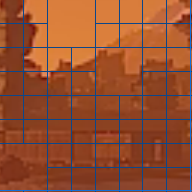
\includegraphics[height=2.5cm]{part_64x64_4.png}\label{fig:jnd-sb-4}}
    \caption{SVT-AV1超级块划分与纹理复杂度}
    \label{fig:jnd-sb}
  \end{figure}

  根据\ref{sec:blk-based-jnd}提出的块级JND感知阈值定义,一个$8\times 8$编码块的感知特征可以通过块级的JND感知阈值$\mathrm{JND_{8x8}}(i, j)$反映,对于更高级别的编码块,其特征变化程度可以通过它的四个编码子块的JND感知阈值差异程度来表现。如式\ref{equ:pi}所示,定义一个编码块的感知划分指标PI为其四个编码子块PI的最大差值。

  \begin{equation} \label{equ:pi}
    \mathrm{PI}(d, k) =
    \begin{dcases}
      \max_{m,n\in \{0, 1, 2, 3\}} \{\mathrm{PI}(d+1, k, m) - \mathrm{PI}(d+1,k, n) \} , &\mathrm{if} \, d \leq 2,\\
      \quad \mathrm{JND_{8x8}}(k), &\mathrm{if}\, d = 2,
    \end{dcases}
  \end{equation}

  其中$d$表示划分深度,$64\times 64$划分深度为0,依次递增到$8\times 8$划分深度为3 ,$k$表示父块序号,$m, n$表示子块相对序号。PI大表明编码子块间特征差异大,更需要对其进行划分,PI小表明编码块内特征差异小,可以考虑提前终止编码块划分结构的搜索。

  \subsubsection{感知划分指标分析}

 使用twitch的10个1080p游戏序列分析超级块划分方式与感知划分指标PI的关系。经过测试分析,以HearthStone序列为例,其划分模式与感知划分指标PI有如图\ref{fig:jnd-part-PI-example}的关系,可以发现,非划分模式的感知划分指标PI相对较小,并且与划分模式的感知划分指标PI具有一定区分性,因此可以通过感知划分指标PI来指导块划分时的提前终止。而相对应的,划分模式的感知划分指标PI的统计特性并不能找到明显的区分性,因此通过感知划分指标PI难以指导块划分时的提前划分。造成这个区别的原因可能是一般来说游戏序列中的平坦区域比较极端化,与提前终止划分的算法契合度高,而纹理复杂区域各有各的特点,共同特性较少。

  % 这张图需要重新画
  \begin{figure}[!htp]
    \centering
    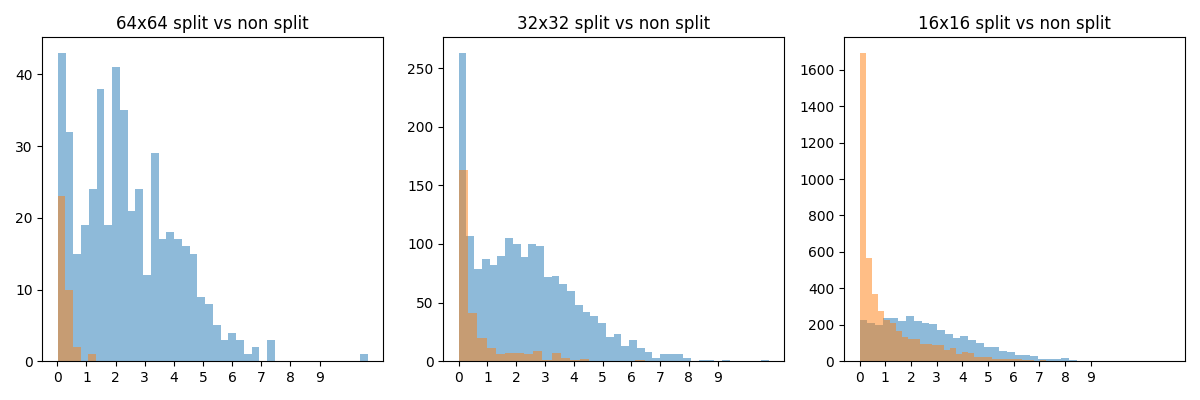
\includegraphics[width=\textwidth]{HEARTHSTONE_part.png}
    \caption{HEARTHSTONE序列划分模式与感知划分指标PI关系图}
   \label{fig:jnd-part-PI-example}
  \end{figure}

	综合分析10个1080p游戏序列,取阈值T为非划分命中率大于50\%的值来均衡加速比与bdrate的损失。另外,考虑到量化参数对块划分的影响,不同QP下应设定不同的阈值PT来提高算法性能。在较小的QP下,视频编码会分配更多的码率,通过更仔细的搜索与块划分来得到更好的重建质量,提前终止划分的感知划分指标PI的阈值PT也相对设定更小。最终的阈值T选择如表\ref{tab:av1-jnd-part-th}所示。

  \begin{table}[!hpt]
    \renewcommand{\arraystretch}{0.9}
    \caption{PI提前终止划分阈值}
    \label{tab:av1-jnd-part-th}
    \centering
    \begin{tabular}{|c|c|c|c|c|c|c|c|c|} \hline
      bsize    & QP & T &bsize    & QP & T&bsize    & QP & T \\ \hline

      \multirow{4}*{$64\times 64$} & 23 & 0.09 &\multirow{4}*{$32\times 32$} & 23 & 0.30 & \multirow{4}*{$16\times 16$} & 23 & 0.40\\ \cline{2-3} \cline{5-6} \cline{8-9}
      & 31 & 0.10 & & 31 & 0.35 & & 31 & 0.45\\ \cline{2-3} \cline{5-6} \cline{8-9}
      & 39 & 0.11 & & 39 & 0.40 & & 39 & 0.50 \\ \cline{2-3} \cline{5-6} \cline{8-9}
      & 47 & 0.13 & & 47 & 0.45 & & 47 & 0.55\\ \hline
    \end{tabular}
  \end{table}

  \subsubsection{快速划分算法结构}

  % 介绍md_stage里面的搜索遍历结构 mds
  如前述章节\ref{sec:pd-md},SVT-AV1使用分阶段决策的方法,包括分阶段分区决策(PD)与分阶段模式选择(MD),在每个MD阶段中,会按照MD的ZigZag扫描方式递归遍历所有划分块的方式,并按照RDCOST的值比较当前块划分与非划分的花费,决策当前块是否划分。利用我们得到的感知划分指标PI,可以在当前块的PI低于一定阈值时,跳过该块的下一深度划分搜索,如\ref{fig:jnd-part-PI-alg}所示。

  \begin{figure}[!htp]
    \centering
    \resizebox{0.6\textwidth}{!}{\begin{tikzpicture}[node distance=2cm]
    \node (input) [startstop] {待划分超级块};
    \node (bsize) [decision, below of=input] {$\mathrm{bsize} \geq 16\mathrm{x}16$};
    \node (PI) [decision, below of=bsize, yshift=-0.8cm] {$\mathrm{PI} < \mathrm{PT_{bsize}}$};
    \node (skip) [process, right of=PI, xshift=3cm] {跳过下一深度划分};
    \node (RDO) [process, below of=PI, yshift=-0.6cm] {RDO};
    \node (end) [startstop, right of=RDO, xshift=3cm] {划分结束};

    %连接具体形状
    \draw [arrow](input) -- (bsize);
    \draw [arrow](bsize) -- node[left] {Yes} (PI);
    \draw [arrow](bsize) -- ($(bsize.west) + (-1.4,0)$) node[above right] {No} |- (RDO);
    \draw [arrow](PI) -- node[left] {No} (RDO);
    \draw [arrow](PI) -- node[above]{Yes} (skip);
    \draw [arrow](skip) |- (bsize);
    \draw [arrow](RDO) -- (end);

\end{tikzpicture}
}
    \caption{感知优化的超级块划分提前终止算法流程图}
    \label{fig:jnd-part-PI-alg}
  \end{figure}

  需要说明的是,因为本文对SVT-AV1的优化是基于其编码器最快预设,在最快预设下,部分AV1的特性被关闭,在块划分上,仅支持最深到$8 \times 8$的正方形划分。

  \subsubsection{调整md-stage进一步优化算法}
  如图\ref{fig:md}所示,SVT-AV1在每个PD阶段中包含多个模式选择MD阶段,在每个MD阶段中会使用各类预测工具与性能指标对各个候选模式进行评估,只留下性能最好的一部分候选,在下一个MD阶段中继续竞争。理论上,多MD阶段决策的最终优化目标是RDO,因为直接计算RDO的计算量较高,在前期的MD阶段中,会使用一些快速算法替代,以牺牲准确性的前提减少了计算量,在最后的MD阶段会使用完整的RDO计算每个候选的RDCOST。在前期快速算法评估下性能较好的候选在完整RDO的评估下的性能可能较差,因此每个MD阶段需要留下一定数量的候选,以防止错失最终性能较好的候选。

  基于JND感知阈值,可以对各阶段的md-stage保留数量做进一步调整以减小计算量。JND感知阈值较高的区域,人眼视觉系统对其失真的敏感度较低,可以适当减小保留的候选数量\texttt{md-stage-count},即使错过最优的候选对视觉效果的影响也比较低。


  \subsection{JND计算的向量加速}

  经过测试,在原始像素级JND模型上计算单帧1080p图像所需的时间超过75ms,对于低延迟编码而言,这个时间是不可接受的,因此将像素级模型简化为块级模型是必要的,使用块级JND模型可以有效减少JND模型的计算量,只需3.4ms左右即可完成一帧的计算,最后,应用SIMD后,可以在此基础上再加速50\%的JND模型运算速度,只需要1.7ms就可以完成对一帧图像的计算。

  \begin{table}[!hpt]
    \renewcommand{\arraystretch}{0.9}
    \caption{1080p单帧图像的JND模型计算测试}
    \label{tab:jnd-compute}
    \centering
    \begin{tabular}{lccc} \toprule
      模型 & ASM & 时间 &时间比  \\ \midrule
      像素级JND模型 & C   & $>75$ms & 100\% \\
      块级JND模型   & C & $\sim 3.4$ms & 4.53\% \\
      块级JND模型   & SSE & $\sim 1.7$ms & 2.27\%\\ \bottomrule
    \end{tabular}
  \end{table}

  为了进一步加速JND部分的计算,对背景亮度计算块和亮度方差使用SIMD进行加速,C代码与intrinsic代码如下。使用SIMD可以拆开C代码中的循环,每次读入块中一行数据,一个指令对8个像素的亮度进行计算。

  \begin{codeblock}[language=C]
/* c code */
uint32_t compute_bg_c(uint8_t *input_samples,
                        uint32_t input_stride,
                        uint32_t input_area_width,
                        uint32_t input_area_height)
{
    uint32_t hi, vi, k = 0;
    uint32_t bg = 0;

    for (vi = 0; vi < input_area_height; vi++) {
        for (hi = 0; hi < input_area_width; hi++) {
            bg += input_samples[hi] * bg_kernel[k++];
        }
        input_samples += input_stride;
    }
    return bg >> 7;
}
/* sse4 intrinsic code */
uint32_t compute_bg8x8_sse4_intrin(
uint8_t *input_samples,
uint32_t input_stride,
uint32_t input_area_width,
uint32_t input_area_height)
{
    __m128i xmm1, xmm2, xmm3, xmm4, xmm_sum, k1, k2, k3, k4;
    k1 = _mm_set_epi16(1, 1, 1, 2, 2, 1, 1, 1);
    k2 = _mm_set_epi16(1, 2, 2, 3, 3, 2, 2, 1);
    k3 = _mm_set_epi16(1, 2, 0, 3, 3, 0, 2, 1);
    k4 = _mm_set_epi16(1, 3, 3, 5, 5, 3, 3, 1);
    xmm1     = _mm_cvtepu8_epi16(_mm_loadl_epi64((__m128i *)(input_samples)));
    xmm2     = _mm_cvtepu8_epi16(_mm_loadl_epi64((__m128i *)(input_samples + input_stride)));
    xmm3     = _mm_cvtepu8_epi16(_mm_loadl_epi64((__m128i *)(input_samples + 2 * input_stride)));
    xmm4     = _mm_cvtepu8_epi16(_mm_loadl_epi64((__m128i *)(input_samples + 3 * input_stride)));
    input_samples += 4 * input_stride;
    xmm4     = _mm_add_epi16(xmm4, _mm_cvtepu8_epi16(_mm_loadl_epi64((__m128i *)(input_samples))));
    xmm3     = _mm_add_epi16(xmm3, _mm_cvtepu8_epi16(_mm_loadl_epi64((__m128i *)(input_samples + input_stride))));
    xmm2     = _mm_add_epi16(xmm2, _mm_cvtepu8_epi16(_mm_loadl_epi64((__m128i *)(input_samples + 2 * input_stride))));
    xmm1     = _mm_add_epi16(xmm1, _mm_cvtepu8_epi16(_mm_loadl_epi64((__m128i *)(input_samples + 3 * input_stride))));
    xmm1     = _mm_mullo_epi16(k1, xmm1);
    xmm2     = _mm_mullo_epi16(k2, xmm2);
    xmm3     = _mm_mullo_epi16(k3, xmm3);
    xmm4     = _mm_mullo_epi16(k4, xmm4);

    xmm1     = _mm_hadd_epi16(xmm1, xmm2);
    xmm3     = _mm_hadd_epi16(xmm3, xmm4);
    xmm_sum = _mm_hadd_epi16(xmm1, xmm3);
    xmm_sum = _mm_hadd_epi16(xmm_sum, xmm_sum);
    xmm_sum = _mm_hadd_epi16(xmm_sum, xmm_sum);
    xmm_sum = _mm_hadd_epi16(xmm_sum, xmm_sum);
    (void)input_area_width;
    (void)input_area_height;

    return (uint32_t)_mm_cvtsi128_si32(xmm_sum) >> 23;
}
  \end{codeblock}
  \subsection{实验结果与分析}

  \subsubsection{实验环境配置}
  实验使用个人笔记本电脑完成,实验系统配置如表\ref{tab:os}所示,实验使用SVT-AV1配置如表\ref{tab:svt}所示,实验测试了All Intra和Low Delay P两种GOP结构,QP取$\{23, 31, 39, 47\}$。编码测试结果包括比特率,PSNR,SSIM,\ref{sec:svt-profile}中提出的SVT-AV1框架的profile工具被用于记录编码时各模块的CPU使用时间,取ENCDEC过程的CPU时间总和作为编码时间来评估算法应用前后的编码复杂度。

  测试序列取twitch的8个1080p游戏序列,一方面游戏直播作为一大重要的直播类型,有着很高的研究价值,另一方面,游戏场景通常是屏幕内容类型的人工场景,场景中简单纹理较多,适合所提算法的测试。

  测试时使用命令\texttt{sudo cpupower frequency-set -g performance}将CPU频率策略调整为“performance”,以确保按照CPU使用时间计算的算法计算量对比准确。

  \begin{table}[!hpt]
    \renewcommand{\arraystretch}{0.9}
    \caption{实验系统配置}
    \label{tab:os}
    \centering
    \begin{tabular}{lc} \toprule
      项目& 参数  \\ \midrule
      OS:     &Manjaro 20.0 Lysia\\
      Kernel: & x86\_64 Linux 5.6.7-1-MANJARO\\
      CPU:    &Intel Core i7-6700HQ @ 8x 3.5GHz\\
      RAM:    &16GB\\
      GCC:    &v9.3.0\\
      SVT-AV1: & v0.8.1\\ \bottomrule
    \end{tabular}
  \end{table}

  \begin{table}[!hpt]
    \renewcommand{\arraystretch}{0.9}
    \caption{SVT-AV1编码器参数配置}
    \label{tab:svt}
    \centering
    \begin{tabular}{lc} \toprule
      项目& 参数  \\ \midrule
      preset     &8\\
      pred-struct& LDP\\
      lookahead    &0\\
      fps    &60\\
      GOP    &60\\
      asm    & up tp avx2\\
      bitdepth & 8\\
      hierarchicalLevels  & 4 \\
      rc & CQP\\ \bottomrule
    \end{tabular}
  \end{table}

  \subsubsection{实验结果分析}

  对算法性能的评估通过测试两种图像质量评价指标完成,分别是峰值信噪比PSNR指标和与结构相似度SSIM指标。
  对算法性能的评估分为两点:

  \begin{enumerate}[label=\arabic*)]
    \item 使用提前终止划分的快速算法带来的编码复杂度降低,通过编码时间节省比例表现;
    \item 算法导致的编码性能下降,通过比特率与峰值信噪比PSNR指标、结构相似度SSIM指标综合分析BDRATE表现。
  \end{enumerate}

  表\ref{tab:av1-jnd-part-AI}、\ref{tab:av1-jnd-part-ldp}分别是在All Intra、Low Delay P预测结构下的实验结果,表\ref{tab:av1-jnd-part-AI-md-stage}是在All Intra预测结构加上调整md\_stage得到的实验结果。

  从实验结果有以下发现:

  \begin{enumerate}[label=\arabic*)]
    \item 对于ALL Intra和Low Delay P两种预测结构,所提算法均可以减少15\%左右的编码时间,其中All Intra的编码时间减少量略高于Low Delay P;
    \item 所提的快速算法会增加编码的码率、减小图像质量,因此BDRATE会有一定程度的上升,其中All Intra的BDRATE增加量少于Low Delay P;
    \item 不同游戏序列的编码时间减少量和BDRATE增加都有所不同,这是因为不同游戏序列的画面纹理特征有较大差异,而我们使用的是一个相对一般化的感知划分指标阈值。
  \end{enumerate}

  需要注意的是,本算法以SVT-AV1编码器的最快预设为基础实现,SVT-AV1本身已经实现了一些用于块划分的快速算法。本算法的编码时间减少量与BDRATE增加量成对抗关系,若选取更激进的感知划分指标阈值,将会以损失更多BDRATE的代价来减少更多的编码时间;同理,若选取更保守的感知划分指标阈值,BDRATE的增加将会减少,但在编码时间上得到的增益也会减小。


  \begin{table}[!hpt]
    \renewcommand{\arraystretch}{0.9}
    \caption{JND快速编码测试结果ALL Intra}
    \label{tab:av1-jnd-part-AI}
    \centering
    \begin{tabular}{|c|c|c|c|c|c|c|c|} \hline
      序列    & QP & $\Delta$T &  $\Delta$Bitrate & $\Delta$PSNR & $\Delta$SSIM & \makecell{BD-RATE\\(PSNR)} & \makecell{BD-RATE\\(SSIM)}\\ \hline

      \multirow{4}*{CSGO} & 23 & -24.98\% & +1.86\% & -0.10 & -0.00011 & \multirow{4}*{+3.88\%} & \multirow{4}*{+3.63\%} \\ \cline{2-6}
      & 31 & -33.25\% & +1.73\% & -0.11 & -0.00011 &  & \\ \cline{2-6}
      & 39 & -29.15\% & +1.65\% & -0.09 & -0.00013 &  & \\ \cline{2-6}
      & 47 & -27.92\% & +1.55\% & -0.08 & -0.00013 &  & \\ \hline
      \multirow{4}*{DOTA2} & 23 & -15.75\% & +0.70\% & -0.10 & -0.00024 & \multirow{4}*{+1.46\%} & \multirow{4}*{+1.87\%} \\ \cline{2-6}
      & 31 & -22.29\% & +0.13\% & -0.08 & -0.00033 &  & \\ \cline{2-6}
      & 39 & -16.84\% & -0.04\% & -0.06 & -0.00040 &  & \\ \cline{2-6}
      & 47 & -14.33\% & +0.06\% & -0.04 & -0.00034 &  & \\ \hline
      \multirow{4}*{EuroTruckSim2} & 23 & -13.45\% & +0.20\% & -0.20 & -0.00045 & \multirow{4}*{+1.43\%} & \multirow{4}*{+2.03\%} \\ \cline{2-6}
      & 31 & -17.37\% & +0.02\% & -0.11 & -0.00044 &  & \\ \cline{2-6}
      & 39 & -9.68\% & -0.05\% & -0.07 & -0.00046 &  & \\ \cline{2-6}
      & 47 & -9.42\% & -0.03\% & -0.05 & -0.00041 &  & \\ \hline
      \multirow{4}*{Fallout4} & 23 & -13.42\% & +0.55\% & -0.05 & -0.00009 & \multirow{4}*{+0.91\%} & \multirow{4}*{+1.15\%} \\ \cline{2-6}
      & 31 & -13.43\% & +0.23\% & -0.05 & -0.00016 &  & \\ \cline{2-6}
      & 39 & -10.32\% & +0.11\% & -0.04 & -0.00021 &  & \\ \cline{2-6}
      & 47 & -12.82\% & +0.06\% & -0.03 & -0.00021 &  & \\ \hline
      \multirow{4}*{GTAV} & 23 & -4.51\% & +0.13\% & -0.05 & -0.00008 & \multirow{4}*{+0.55\%} & \multirow{4}*{+0.59\%} \\ \cline{2-6}
      & 31 & -21.02\% & +0.05\% & -0.03 & -0.00010 &  & \\ \cline{2-6}
      & 39 & -9.55\% & -0.01\% & -0.03 & -0.00015 &  & \\ \cline{2-6}
      & 47 & -16.22\% & -0.02\% & -0.02 & -0.00015 &  & \\ \hline
      \multirow{4}*{Hearthstone} & 23 & -20.03\% & +0.10\% & -0.01 & -0.00003 & \multirow{4}*{+0.29\%} & \multirow{4}*{+0.63\%} \\ \cline{2-6}
      & 31 & -17.56\% & +0.04\% & -0.02 & -0.00006 &  & \\ \cline{2-6}
      & 39 & -17.02\% & +0.04\% & -0.02 & -0.00009 &  & \\ \cline{2-6}
      & 47 & -9.94\% & +0.01\% & -0.02 & -0.00010 &  & \\ \hline
      \multirow{4}*{MINECRAFT} & 23 & -4.90\% & +0.71\% & -0.11 & -0.00013 & \multirow{4}*{+1.09\%} & \multirow{4}*{+1.16\%} \\ \cline{2-6}
      & 31 & -9.00\% & +0.40\% & -0.09 & -0.00017 &  & \\ \cline{2-6}
      & 39 & -8.78\% & +0.18\% & -0.07 & -0.00024 &  & \\ \cline{2-6}
      & 47 & -11.04\% & +0.08\% & -0.05 & -0.00025 &  & \\ \hline
      \multirow{4}*{RUST} & 23 & -25.32\% & -0.57\% & -0.28 & -0.00066 & \multirow{4}*{+1.70\%} & \multirow{4}*{+1.74\%} \\ \cline{2-6}
      & 31 & -24.67\% & +0.06\% & -0.12 & -0.00038 &  & \\ \cline{2-6}
      & 39 & -25.06\% & -0.08\% & -0.10 & -0.00050 &  & \\ \cline{2-6}
      & 47 & -21.98\% & -0.20\% & -0.07 & -0.00059 &  & \\ \hline
      \multirow{4}*{STARCRAFT} & 23 & -9.29\% & +1.69\% & -0.10 & -0.00018 & \multirow{4}*{+2.15\%} & \multirow{4}*{+3.04\%} \\ \cline{2-6}
      & 31 & -14.63\% & +0.98\% & -0.11 & -0.00031 &  & \\ \cline{2-6}
      & 39 & -13.79\% & +0.59\% & -0.09 & -0.00043 &  & \\ \cline{2-6}
      & 47 & -15.10\% & +0.47\% & -0.06 & -0.00040 &  & \\ \hline
      \multirow{4}*{WITCHER3} & 23 & -20.09\% & +0.77\% & -0.21 & -0.00050 & \multirow{4}*{+2.82\%} & \multirow{4}*{+2.82\%} \\ \cline{2-6}
      & 31 & -22.96\% & +0.34\% & -0.15 & -0.00065 &  & \\ \cline{2-6}
      & 39 & -25.36\% & -0.22\% & -0.14 & -0.00104 &  & \\ \cline{2-6}
      & 47 & -23.16\% & -0.36\% & -0.10 & -0.00111 &  & \\ \hline
      \multicolumn{2}{|c|}{平均值} & -16.89\% & +0.35\% & -0.08 & -0.00031 & +1.63\% & +1.87\%

      \\\hline
    \end{tabular}
  \end{table}

  \begin{table}[!hpt]
    \renewcommand{\arraystretch}{0.9}
    \caption{JND快速编码测试结果Low Delay P}
    \label{tab:av1-jnd-part-ldp}
    \centering
    \begin{tabular}{|c|c|c|c|c|c|c|c|} \hline
      序列    & QP & $\Delta$T &  $\Delta$Bitrate & $\Delta$PSNR & $\Delta$SSIM & \makecell{BD-RATE\\(PSNR)} & \makecell{BD-RATE\\(SSIM)}\\ \hline

      \multirow{4}*{CSGO} & 23 & -24.59\% & -0.17\% & -0.13 & -0.00026 & \multirow{4}*{+3.12\%} & \multirow{4}*{+3.29\%} \\ \cline{2-6}
      & 31 & -26.33\% & +0.80\% & -0.08 & -0.00017 &  & \\ \cline{2-6}
      & 39 & -19.99\% & +1.35\% & -0.07 & -0.00018 &  & \\ \cline{2-6}
      & 47 & -26.84\% & +1.90\% & -0.05 & -0.00016 &  & \\ \hline
      \multirow{4}*{DOTA2} & 23 & -13.68\% & +0.97\% & -0.09 & -0.00048 & \multirow{4}*{+2.37\%} & \multirow{4}*{+3.42\%} \\ \cline{2-6}
      & 31 & -14.37\% & +0.25\% & -0.07 & -0.00048 &  & \\ \cline{2-6}
      & 39 & -16.17\% & -0.01\% & -0.05 & -0.00055 &  & \\ \cline{2-6}
      & 47 & -16.77\% & -0.03\% & -0.04 & -0.00046 &  & \\ \hline
      \multirow{4}*{EuroTruckSim2} & 23 & -7.95\% & +0.45\% & -0.05 & -0.00036 & \multirow{4}*{+1.53\%} & \multirow{4}*{+3.23\%} \\ \cline{2-6}
      & 31 & -6.41\% & +0.29\% & -0.06 & -0.00068 &  & \\ \cline{2-6}
      & 39 & -7.82\% & +0.21\% & -0.06 & -0.00092 &  & \\ \cline{2-6}
      & 47 & -10.69\% & +0.16\% & -0.03 & -0.00079 &  & \\ \hline
      \multirow{4}*{Fallout4} & 23 & -5.75\% & +0.35\% & -0.04 & -0.00024 & \multirow{4}*{+1.09\%} & \multirow{4}*{+1.92\%} \\ \cline{2-6}
      & 31 & -8.01\% & +0.23\% & -0.03 & -0.00029 &  & \\ \cline{2-6}
      & 39 & -9.70\% & +0.07\% & -0.03 & -0.00041 &  & \\ \cline{2-6}
      & 47 & -10.98\% & +0.25\% & -0.02 & -0.00045 &  & \\ \hline
      \multirow{4}*{GTAV} & 23 & -8.56\% & +0.75\% & -0.04 & -0.00026 & \multirow{4}*{+2.32\%} & \multirow{4}*{+3.39\%} \\ \cline{2-6}
      & 31 & -11.10\% & +1.15\% & -0.05 & -0.00042 &  & \\ \cline{2-6}
      & 39 & -10.55\% & +0.38\% & -0.03 & -0.00048 &  & \\ \cline{2-6}
      & 47 & -10.16\% & +0.12\% & -0.04 & -0.00054 &  & \\ \hline
      \multirow{4}*{Hearthstone} & 23 & -10.97\% & -0.52\% & -0.03 & -0.00006 & \multirow{4}*{+0.42\%} & \multirow{4}*{+0.95\%} \\ \cline{2-6}
      & 31 & -10.41\% & +0.21\% & -0.01 & -0.00006 &  & \\ \cline{2-6}
      & 39 & -10.33\% & +0.25\% & -0.02 & -0.00008 &  & \\ \cline{2-6}
      & 47 & -9.43\% & +0.07\% & -0.02 & -0.00013 &  & \\ \hline
      \multirow{4}*{MINECRAFT} & 23 & -4.88\% & +0.30\% & -0.06 & -0.00029 & \multirow{4}*{+1.11\%} & \multirow{4}*{+1.34\%} \\ \cline{2-6}
      & 31 & -4.16\% & +0.24\% & -0.06 & -0.00045 &  & \\ \cline{2-6}
      & 39 & -5.86\% & +0.30\% & -0.04 & -0.00061 &  & \\ \cline{2-6}
      & 47 & -6.91\% & -0.16\% & -0.04 & -0.00081 &  & \\ \hline
      \multirow{4}*{RUST} & 23 & -15.99\% & +0.89\% & -0.10 & -0.00075 & \multirow{4}*{+3.03\%} & \multirow{4}*{+3.78\%} \\ \cline{2-6}
      & 31 & -17.93\% & +1.31\% & -0.06 & -0.00072 &  & \\ \cline{2-6}
      & 39 & -17.50\% & +0.14\% & -0.07 & -0.00123 &  & \\ \cline{2-6}
      & 47 & -20.22\% & -0.62\% & -0.06 & -0.00154 &  & \\ \hline
      \multirow{4}*{STARCRAFT} & 23 & -9.06\% & +1.17\% & -0.06 & -0.00028 & \multirow{4}*{+1.72\%} & \multirow{4}*{+2.71\%} \\ \cline{2-6}
      & 31 & -9.53\% & +0.71\% & -0.06 & -0.00041 &  & \\ \cline{2-6}
      & 39 & -9.31\% & +0.20\% & -0.06 & -0.00055 &  & \\ \cline{2-6}
      & 47 & -9.76\% & +0.52\% & -0.03 & -0.00051 &  & \\ \hline
      \multirow{4}*{WITCHER3} & 23 & -18.55\% & +0.42\% & -0.12 & -0.00113 & \multirow{4}*{+3.82\%} & \multirow{4}*{+3.91\%} \\ \cline{2-6}
      & 31 & -21.62\% & +0.04\% & -0.12 & -0.00168 &  & \\ \cline{2-6}
      & 39 & -17.42\% & -0.70\% & -0.09 & -0.00162 &  & \\ \cline{2-6}
      & 47 & -20.60\% & -1.18\% & -0.04 & -0.00092 &  & \\ \hline
      \multicolumn{2}{|c|}{平均值} & -12.92\% & +0.33\% & -0.06 & -0.00056 & +2.05\% & +2.79\%

       \\\hline
    \end{tabular}
  \end{table}

  \begin{table}[!hpt]
    \renewcommand{\arraystretch}{0.9}
    \caption{调整md-stage进一步优化JND快速编码测试结果All Intra}
    \label{tab:av1-jnd-part-AI-md-stage}
    \centering
    \begin{tabular}{|c|c|c|c|c|c|c|c|} \hline
      序列    & QP & $\Delta$T &  $\Delta$Bitrate & $\Delta$PSNR & $\Delta$SSIM & \makecell{BD-RATE\\(PSNR)} & \makecell{BD-RATE\\(SSIM)}\\ \hline

      \multirow{4}*{CSGO} & 23 & -49.01\% & +2.23\% & -0.13 & -0.00014 & \multirow{4}*{+4.78\%} & \multirow{4}*{+4.88\%} \\ \cline{2-6}
      & 31 & -46.94\% & +1.86\% & -0.13 & -0.00016 &  & \\ \cline{2-6}
      & 39 & -44.36\% & +1.88\% & -0.13 & -0.00021 &  & \\ \cline{2-6}
      & 47 & -40.54\% & +1.99\% & -0.12 & -0.00023 &  & \\ \hline
      \multirow{4}*{DOTA2} & 23 & -35.24\% & +0.91\% & -0.11 & -0.00026 & \multirow{4}*{+1.87\%} & \multirow{4}*{+2.39\%} \\ \cline{2-6}
      & 31 & -38.34\% & +0.32\% & -0.09 & -0.00037 &  & \\ \cline{2-6}
      & 39 & -30.65\% & +0.03\% & -0.09 & -0.00052 &  & \\ \cline{2-6}
      & 47 & -31.13\% & +0.18\% & -0.06 & -0.00050 &  & \\ \hline
      \multirow{4}*{EuroTruckSim2} & 23 & -36.84\% & +0.31\% & -0.23 & -0.00048 & \multirow{4}*{+1.81\%} & \multirow{4}*{+2.31\%} \\ \cline{2-6}
      & 31 & -34.28\% & +0.14\% & -0.13 & -0.00045 &  & \\ \cline{2-6}
      & 39 & -27.65\% & -0.05\% & -0.09 & -0.00054 &  & \\ \cline{2-6}
      & 47 & -27.67\% & -0.06\% & -0.07 & -0.00055 &  & \\ \hline
      \multirow{4}*{Fallout4} & 23 & -29.81\% & +0.89\% & -0.07 & -0.00011 & \multirow{4}*{+1.53\%} & \multirow{4}*{+1.82\%} \\ \cline{2-6}
      & 31 & -29.64\% & +0.50\% & -0.07 & -0.00021 &  & \\ \cline{2-6}
      & 39 & -22.24\% & +0.38\% & -0.07 & -0.00030 &  & \\ \cline{2-6}
      & 47 & -23.67\% & +0.34\% & -0.06 & -0.00037 &  & \\ \hline
      \multirow{4}*{GTAV} & 23 & -28.42\% & +0.30\% & -0.07 & -0.00012 & \multirow{4}*{+1.04\%} & \multirow{4}*{+1.10\%} \\ \cline{2-6}
      & 31 & -32.79\% & +0.07\% & -0.06 & -0.00018 &  & \\ \cline{2-6}
      & 39 & -26.01\% & -0.03\% & -0.06 & -0.00029 &  & \\ \cline{2-6}
      & 47 & -31.04\% & -0.03\% & -0.05 & -0.00035 &  & \\ \hline
      \multirow{4}*{Hearthstone} & 23 & -35.88\% & +0.41\% & -0.03 & -0.00006 & \multirow{4}*{+0.81\%} & \multirow{4}*{+1.37\%} \\ \cline{2-6}
      & 31 & -31.95\% & +0.24\% & -0.05 & -0.00011 &  & \\ \cline{2-6}
      & 39 & -27.62\% & +0.24\% & -0.05 & -0.00018 &  & \\ \cline{2-6}
      & 47 & -25.36\% & +0.22\% & -0.04 & -0.00020 &  & \\ \hline
      \multirow{4}*{MINECRAFT} & 23 & -25.34\% & +0.68\% & -0.13 & -0.00015 & \multirow{4}*{+1.17\%} & \multirow{4}*{+1.26\%} \\ \cline{2-6}
      & 31 & -25.46\% & +0.26\% & -0.11 & -0.00021 &  & \\ \cline{2-6}
      & 39 & -23.94\% & +0.08\% & -0.09 & -0.00030 &  & \\ \cline{2-6}
      & 47 & -25.77\% & +0.05\% & -0.06 & -0.00031 &  & \\ \hline
      \multirow{4}*{RUST} & 23 & -40.12\% & -0.31\% & -0.32 & -0.00075 & \multirow{4}*{+2.04\%} & \multirow{4}*{+2.13\%} \\ \cline{2-6}
      & 31 & -37.87\% & +0.04\% & -0.15 & -0.00050 &  & \\ \cline{2-6}
      & 39 & -37.09\% & -0.17\% & -0.12 & -0.00062 &  & \\ \cline{2-6}
      & 47 & -33.71\% & -0.35\% & -0.09 & -0.00074 &  & \\ \hline
      \multirow{4}*{STARCRAFT} & 23 & -30.98\% & +1.85\% & -0.12 & -0.00020 & \multirow{4}*{+2.50\%} & \multirow{4}*{+3.47\%} \\ \cline{2-6}
      & 31 & -29.00\% & +1.09\% & -0.12 & -0.00034 &  & \\ \cline{2-6}
      & 39 & -30.69\% & +0.72\% & -0.11 & -0.00050 &  & \\ \cline{2-6}
      & 47 & -29.44\% & +0.64\% & -0.08 & -0.00049 &  & \\ \hline
      \multirow{4}*{WITCHER3} & 23 & -38.68\% & +0.74\% & -0.23 & -0.00053 & \multirow{4}*{+2.97\%} & \multirow{4}*{+2.97\%} \\ \cline{2-6}
      & 31 & -40.61\% & +0.22\% & -0.16 & -0.00071 &  & \\ \cline{2-6}
      & 39 & -39.68\% & -0.38\% & -0.15 & -0.00115 &  & \\ \cline{2-6}
      & 47 & -37.01\% & -0.60\% & -0.12 & -0.00132 &  & \\ \hline
      \multicolumn{2}{|c|}{平均值} & -32.81\% & +0.45\% & -0.11 & -0.00039 & +2.05\% & +2.37\%

       \\\hline
    \end{tabular}
  \end{table}

  \subsubsection{实验结果主观评估}

  图\ref{fig:dota2-part}展示了在DOTA2序列上,原始算法与所提算法的超级块划分对比图,其中图\ref{fig:dota2-origin-part}展示了SVT-AV1原始算法的超级块划分,图\ref{fig:dota2-jnd-part}展示了应用基于JND的快速划分算法后的超级块划分效果,图\ref{fig:dota2-md-part}展示了基于JND调整md-stage的快速划分算法后的超级块划分效果。对比发现,在纹理简单、一致性较高的区域,应用了所提算法后,更倾向于划分较大的块;对于纹理复杂的区域,二者的划分比较一致,均有细致的分块。

  \begin{figure}[!hbtp]
    \setlength\abovecaptionskip{-0.05cm}
    \centering
    \subcaptionbox{原始算法超级块划分图\label{fig:dota2-origin-part}}
                    [\textwidth]{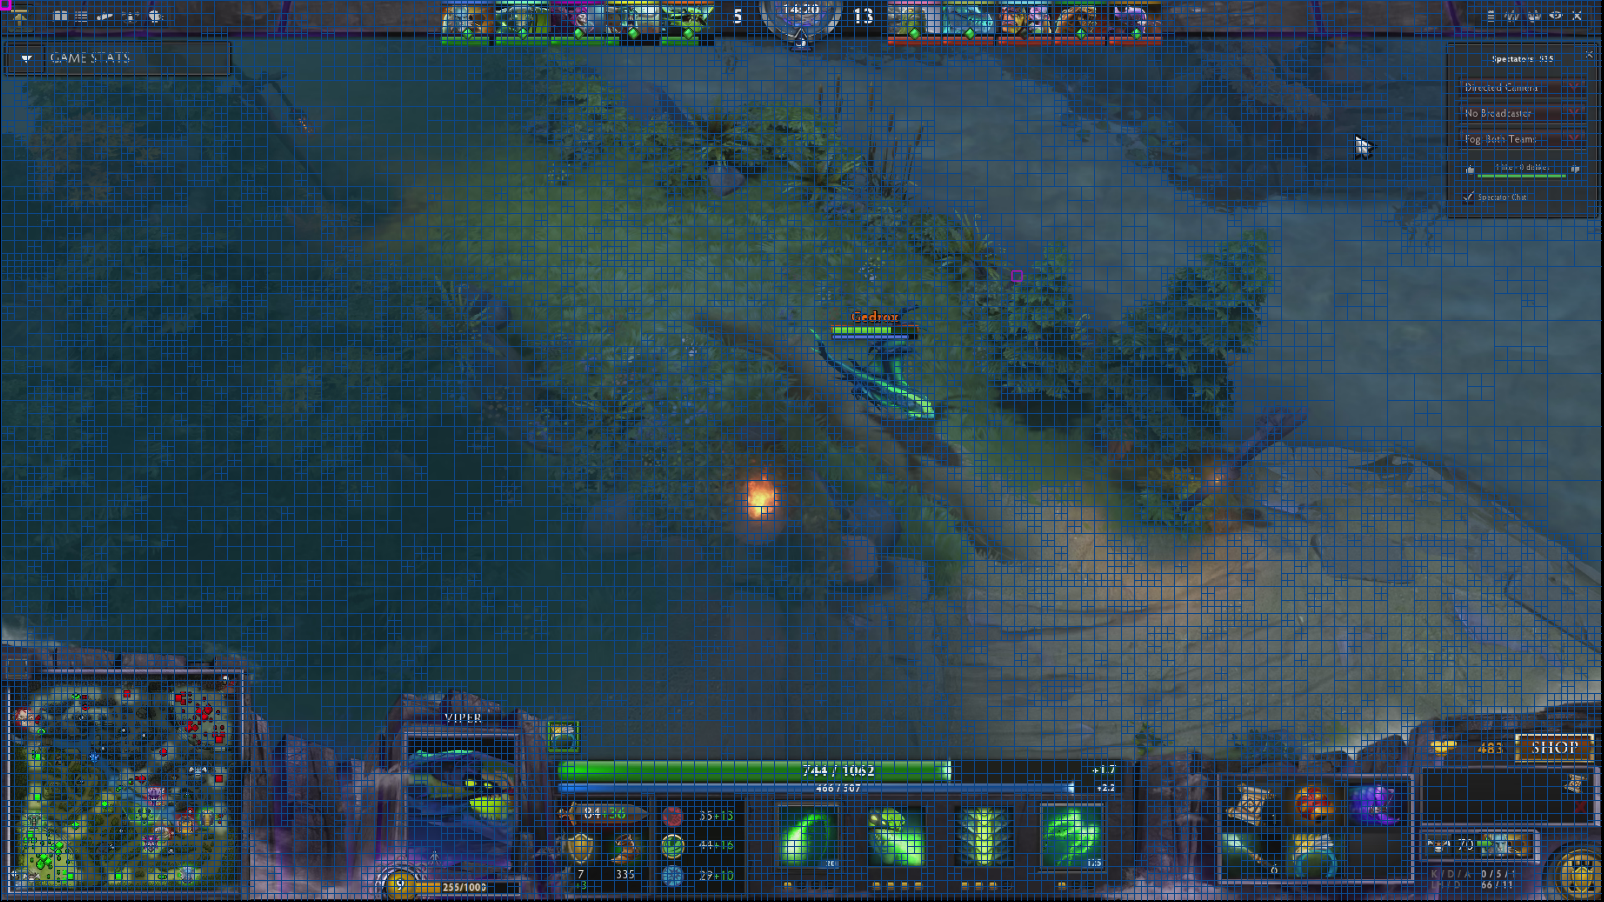
\includegraphics[width=0.885\textwidth]{dota2_origin_partition.png}}
    \subcaptionbox{JND优化快速算法超级块划分图\label{fig:dota2-jnd-part}}
                    [\textwidth]{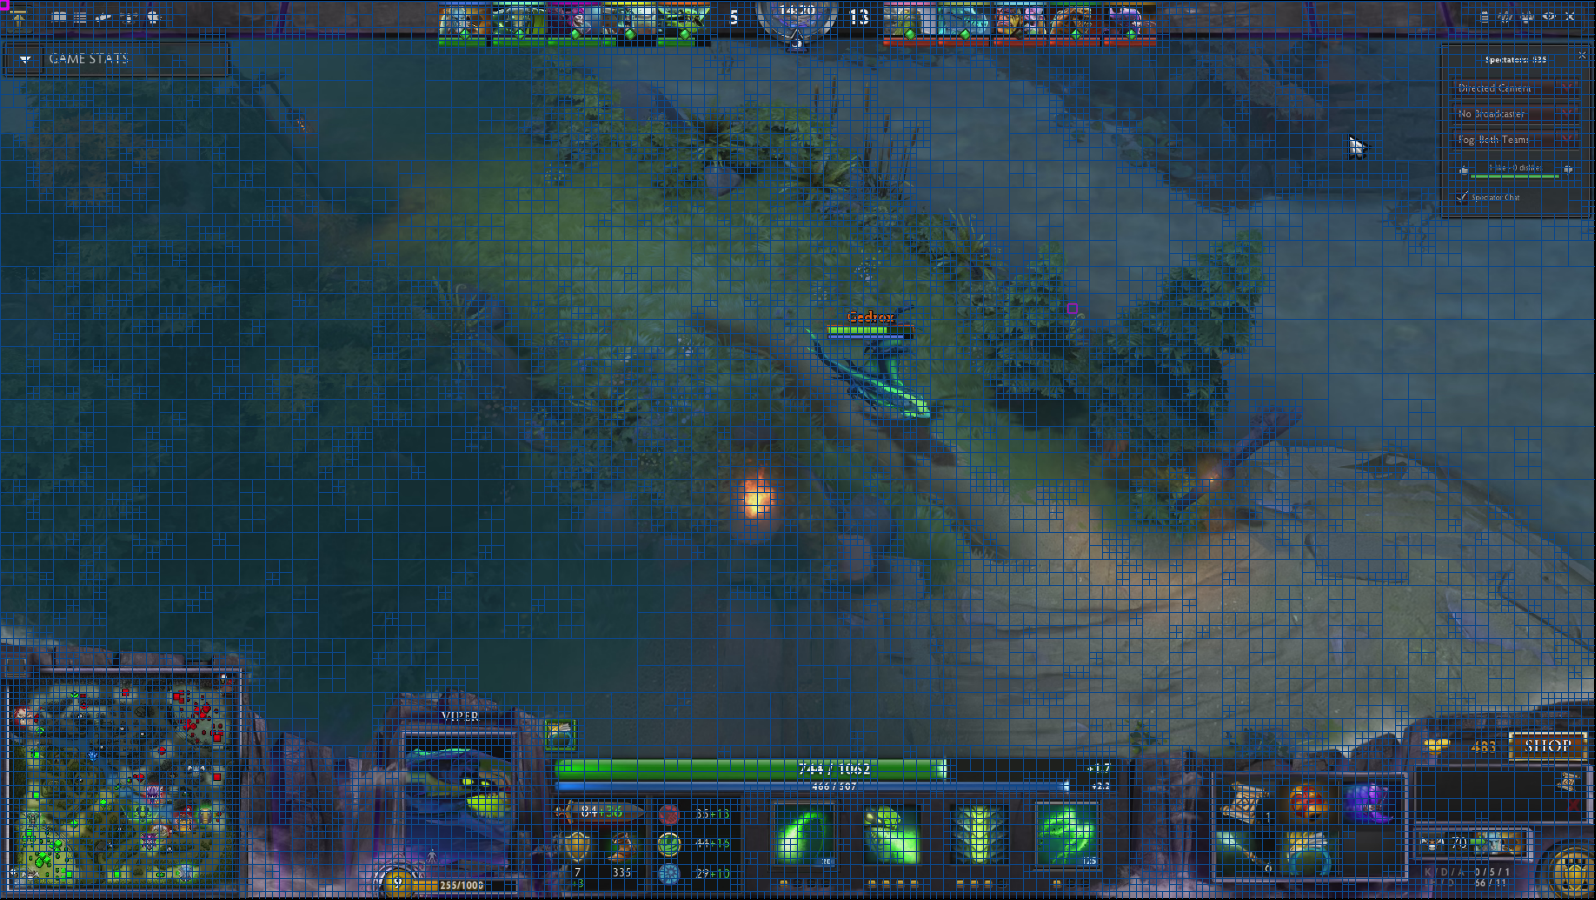
\includegraphics[width=0.885\textwidth]{dota2_jnd_partition.png}}
    \subcaptionbox{md-stage调整的JND优化快速算法超级块划分图\label{fig:dota2-md-part}}
                    [\textwidth]{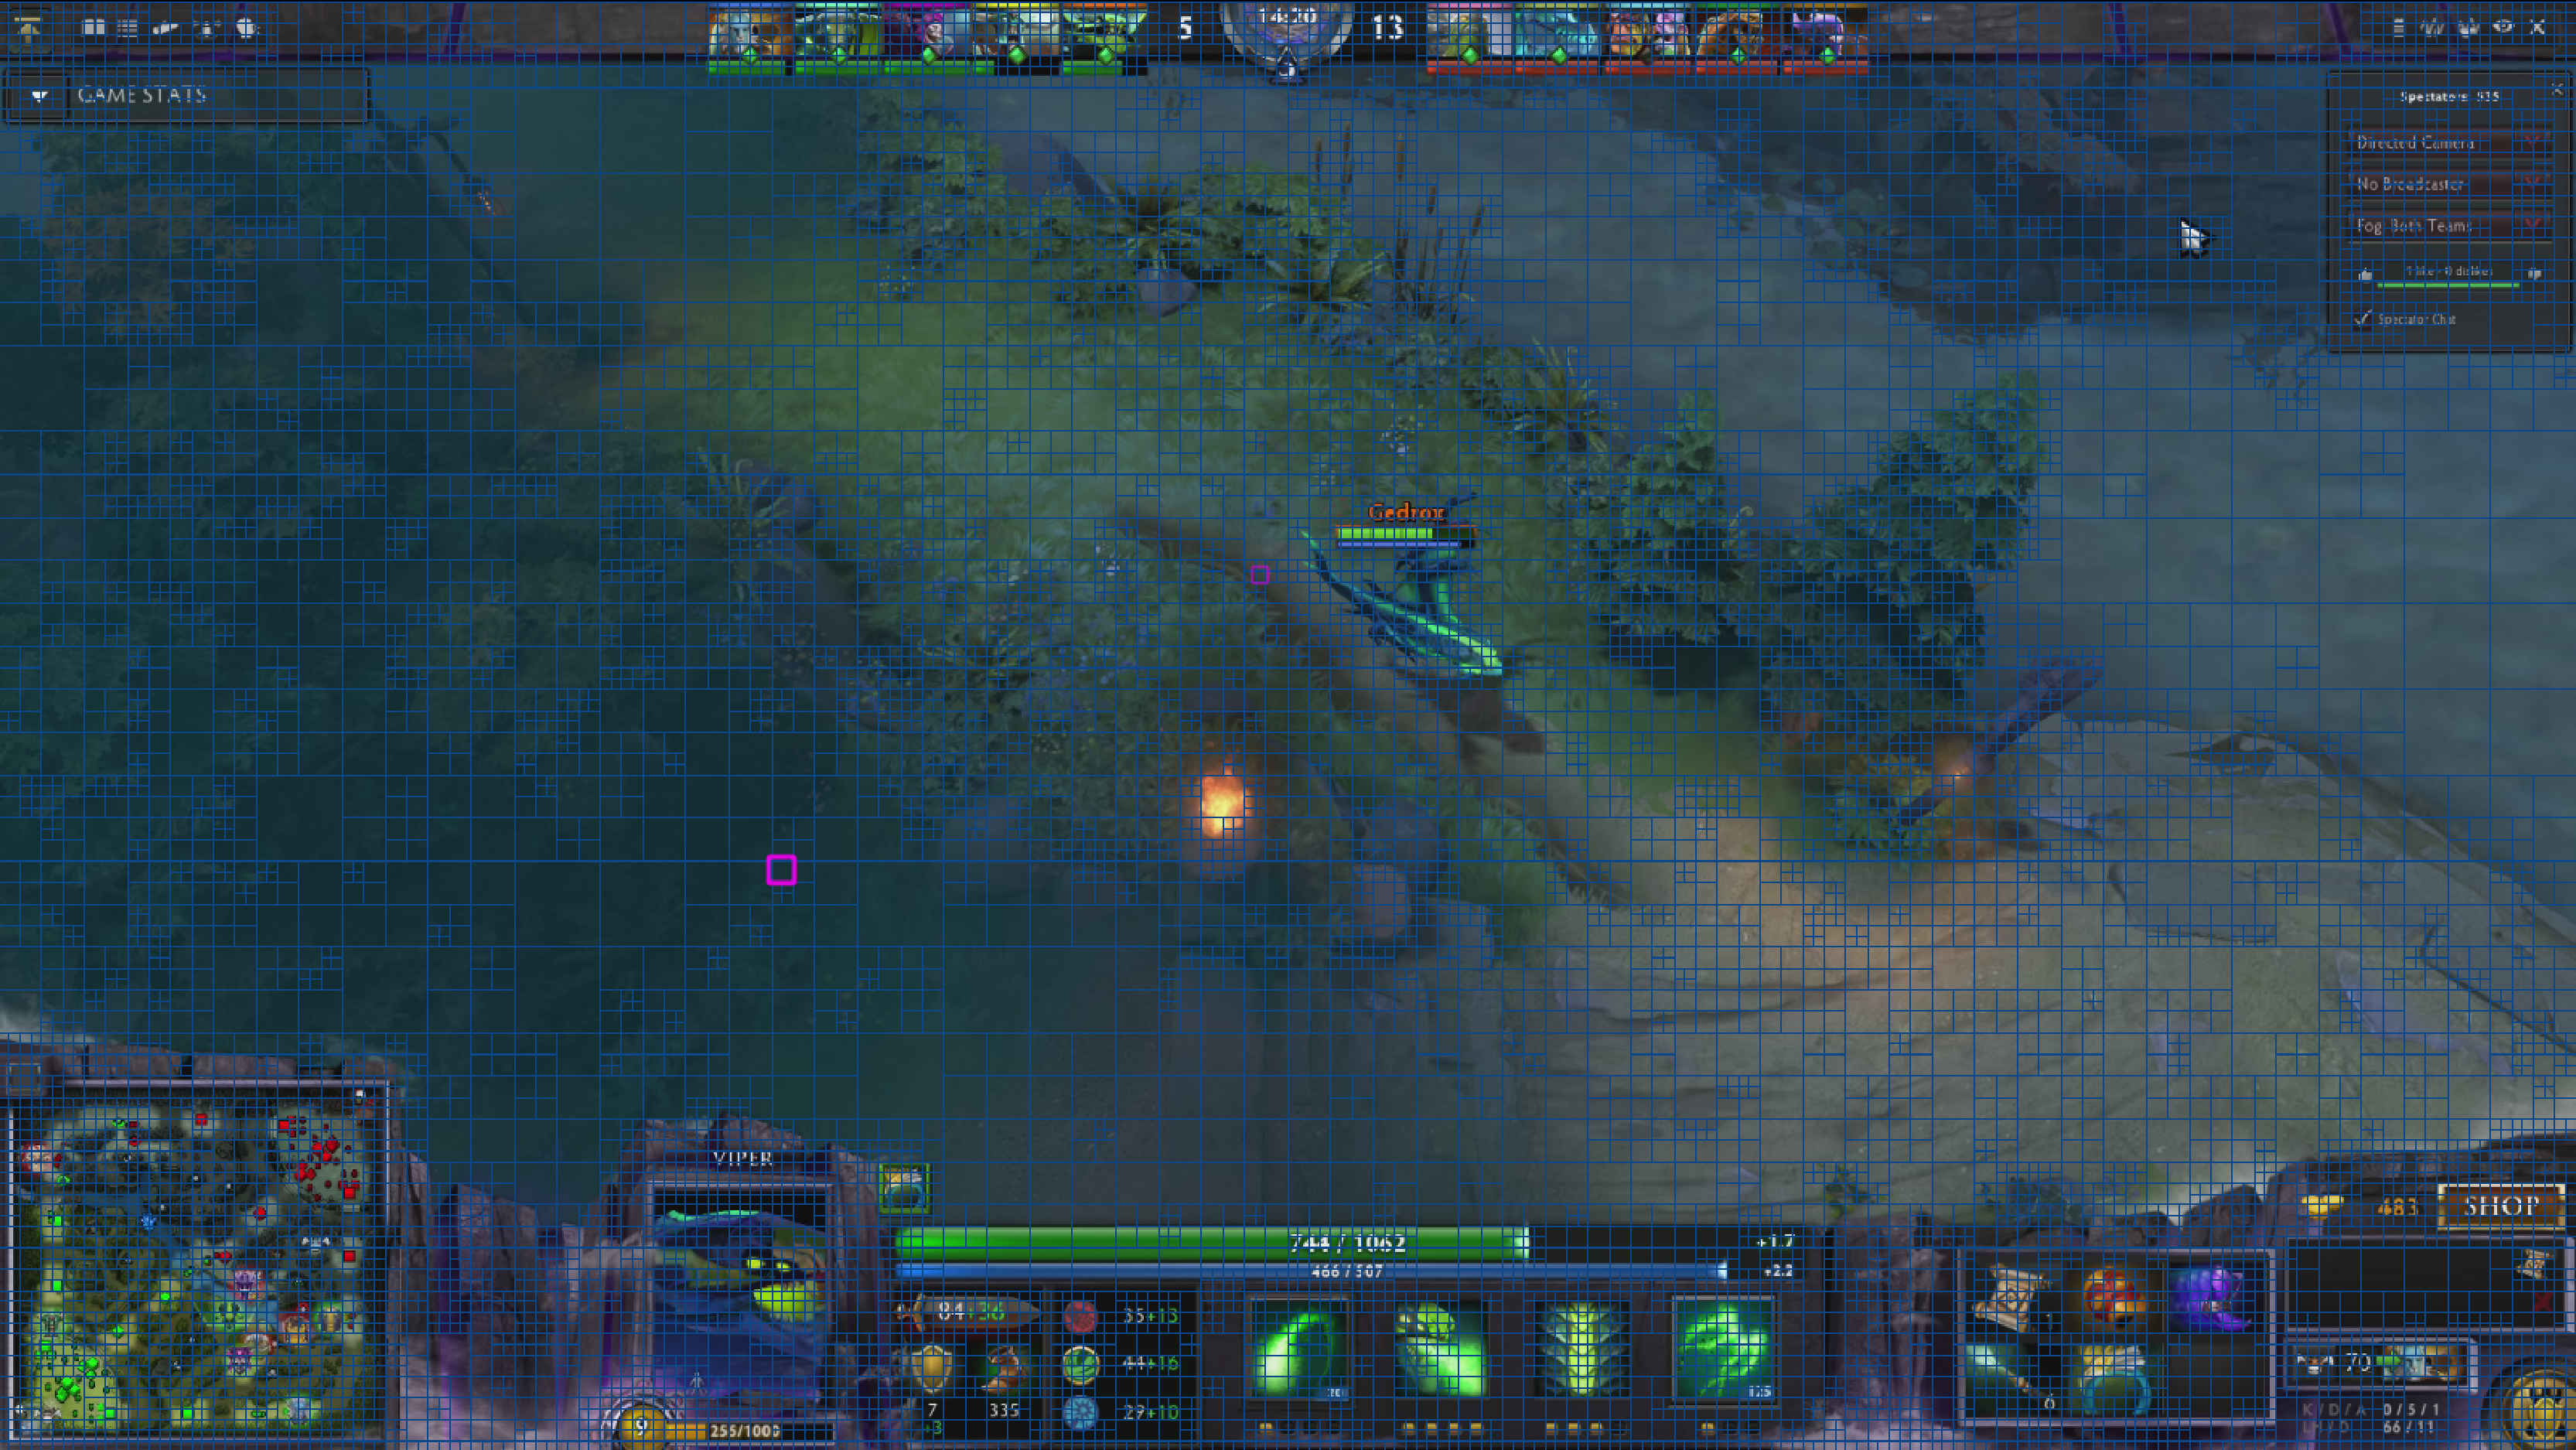
\includegraphics[width=0.885\textwidth]{dota2_md_partition.png}}
    \caption{原始算法与所提算法的超级块划分对比图}
    \label{fig:dota2-part}
  \end{figure}

  图\ref{fig:dota2-decode}展示了在DOTA2序列上,原始算法与所提算法的解码图像对比,其中图\ref{fig:dota2-origin-dec}展示了SVT-AV1原始算法的解码图像,图\ref{fig:dota2-jnd-dec}展示了应用基于JND的快速划分算法后的解码图像,图\ref{fig:dota2-md-dec}展示了应用基于JND调整md-stage的快速划分算法后的解码图像。对比发现,使用所提算法对主观质量基本没有影响。

  \begin{figure}[!hbtp]
    \setlength\abovecaptionskip{-0.05cm}
    \centering
    \subcaptionbox{原始算法解码图像\label{fig:dota2-origin-dec}}
                    [\textwidth]{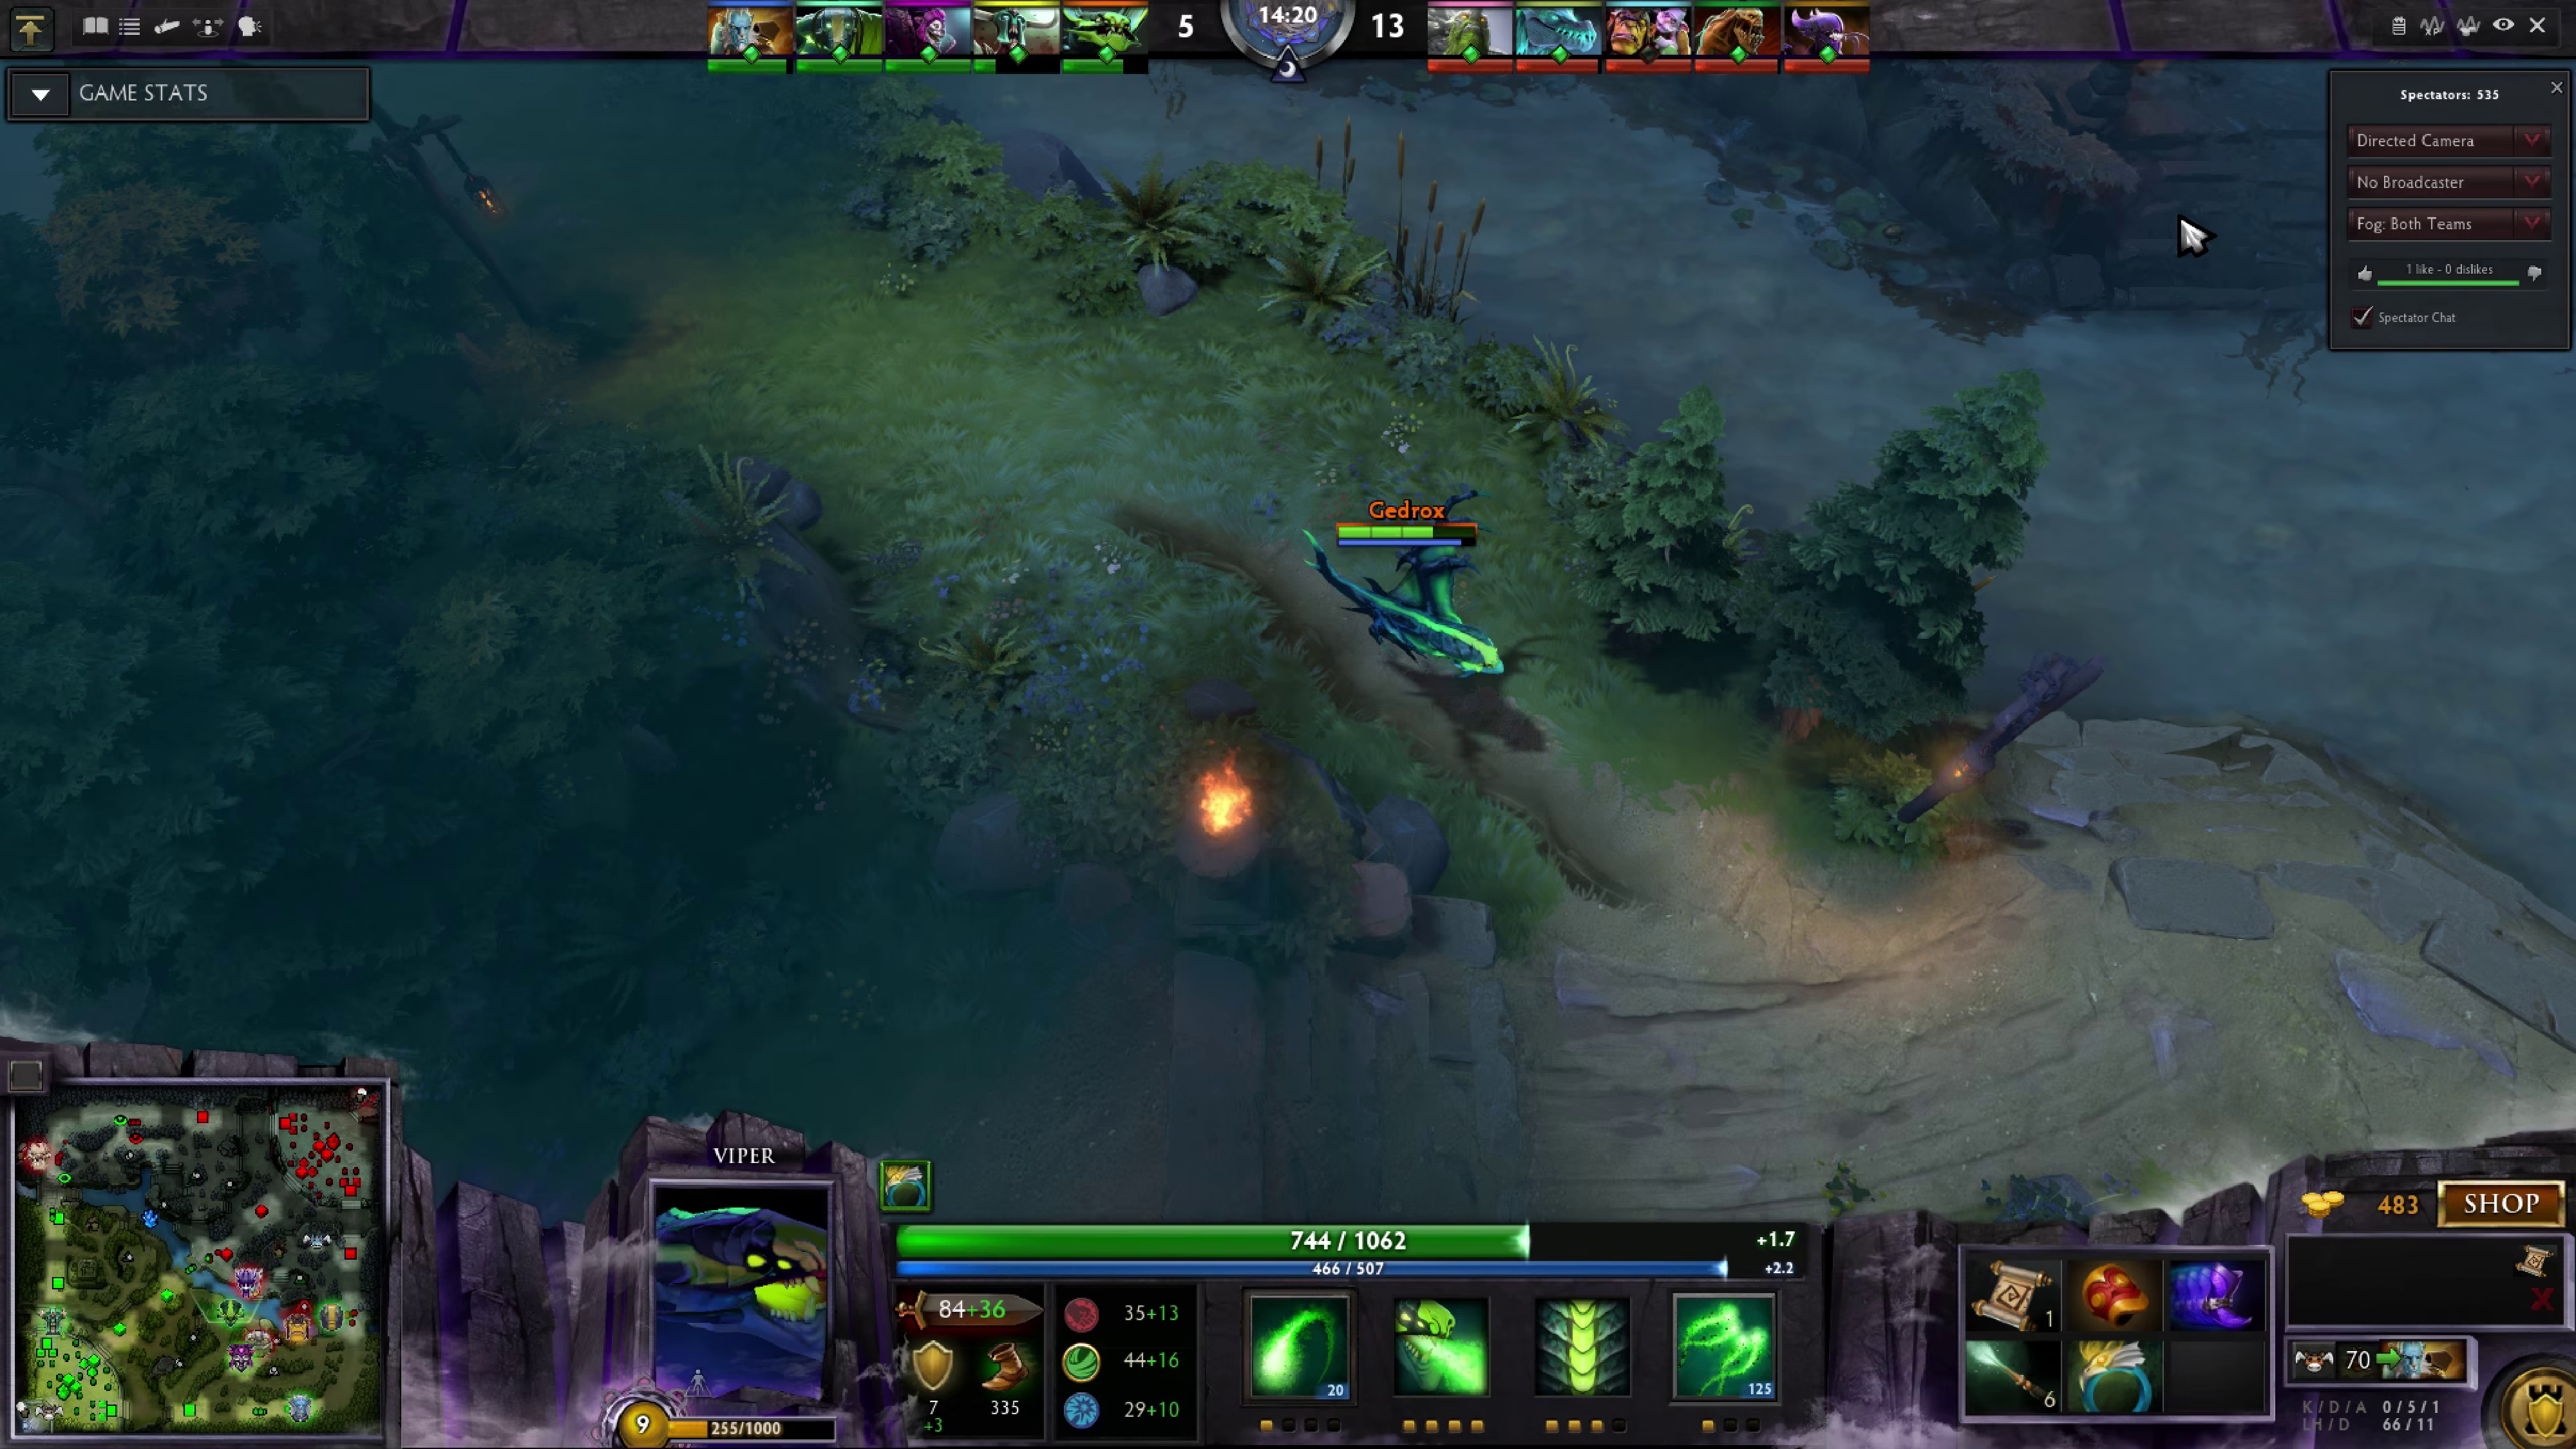
\includegraphics[width=0.885\textwidth]{dota2_origin_decode.png}}
    \subcaptionbox{所提算法解码图像\label{fig:dota2-jnd-dec}}
                    [\textwidth]{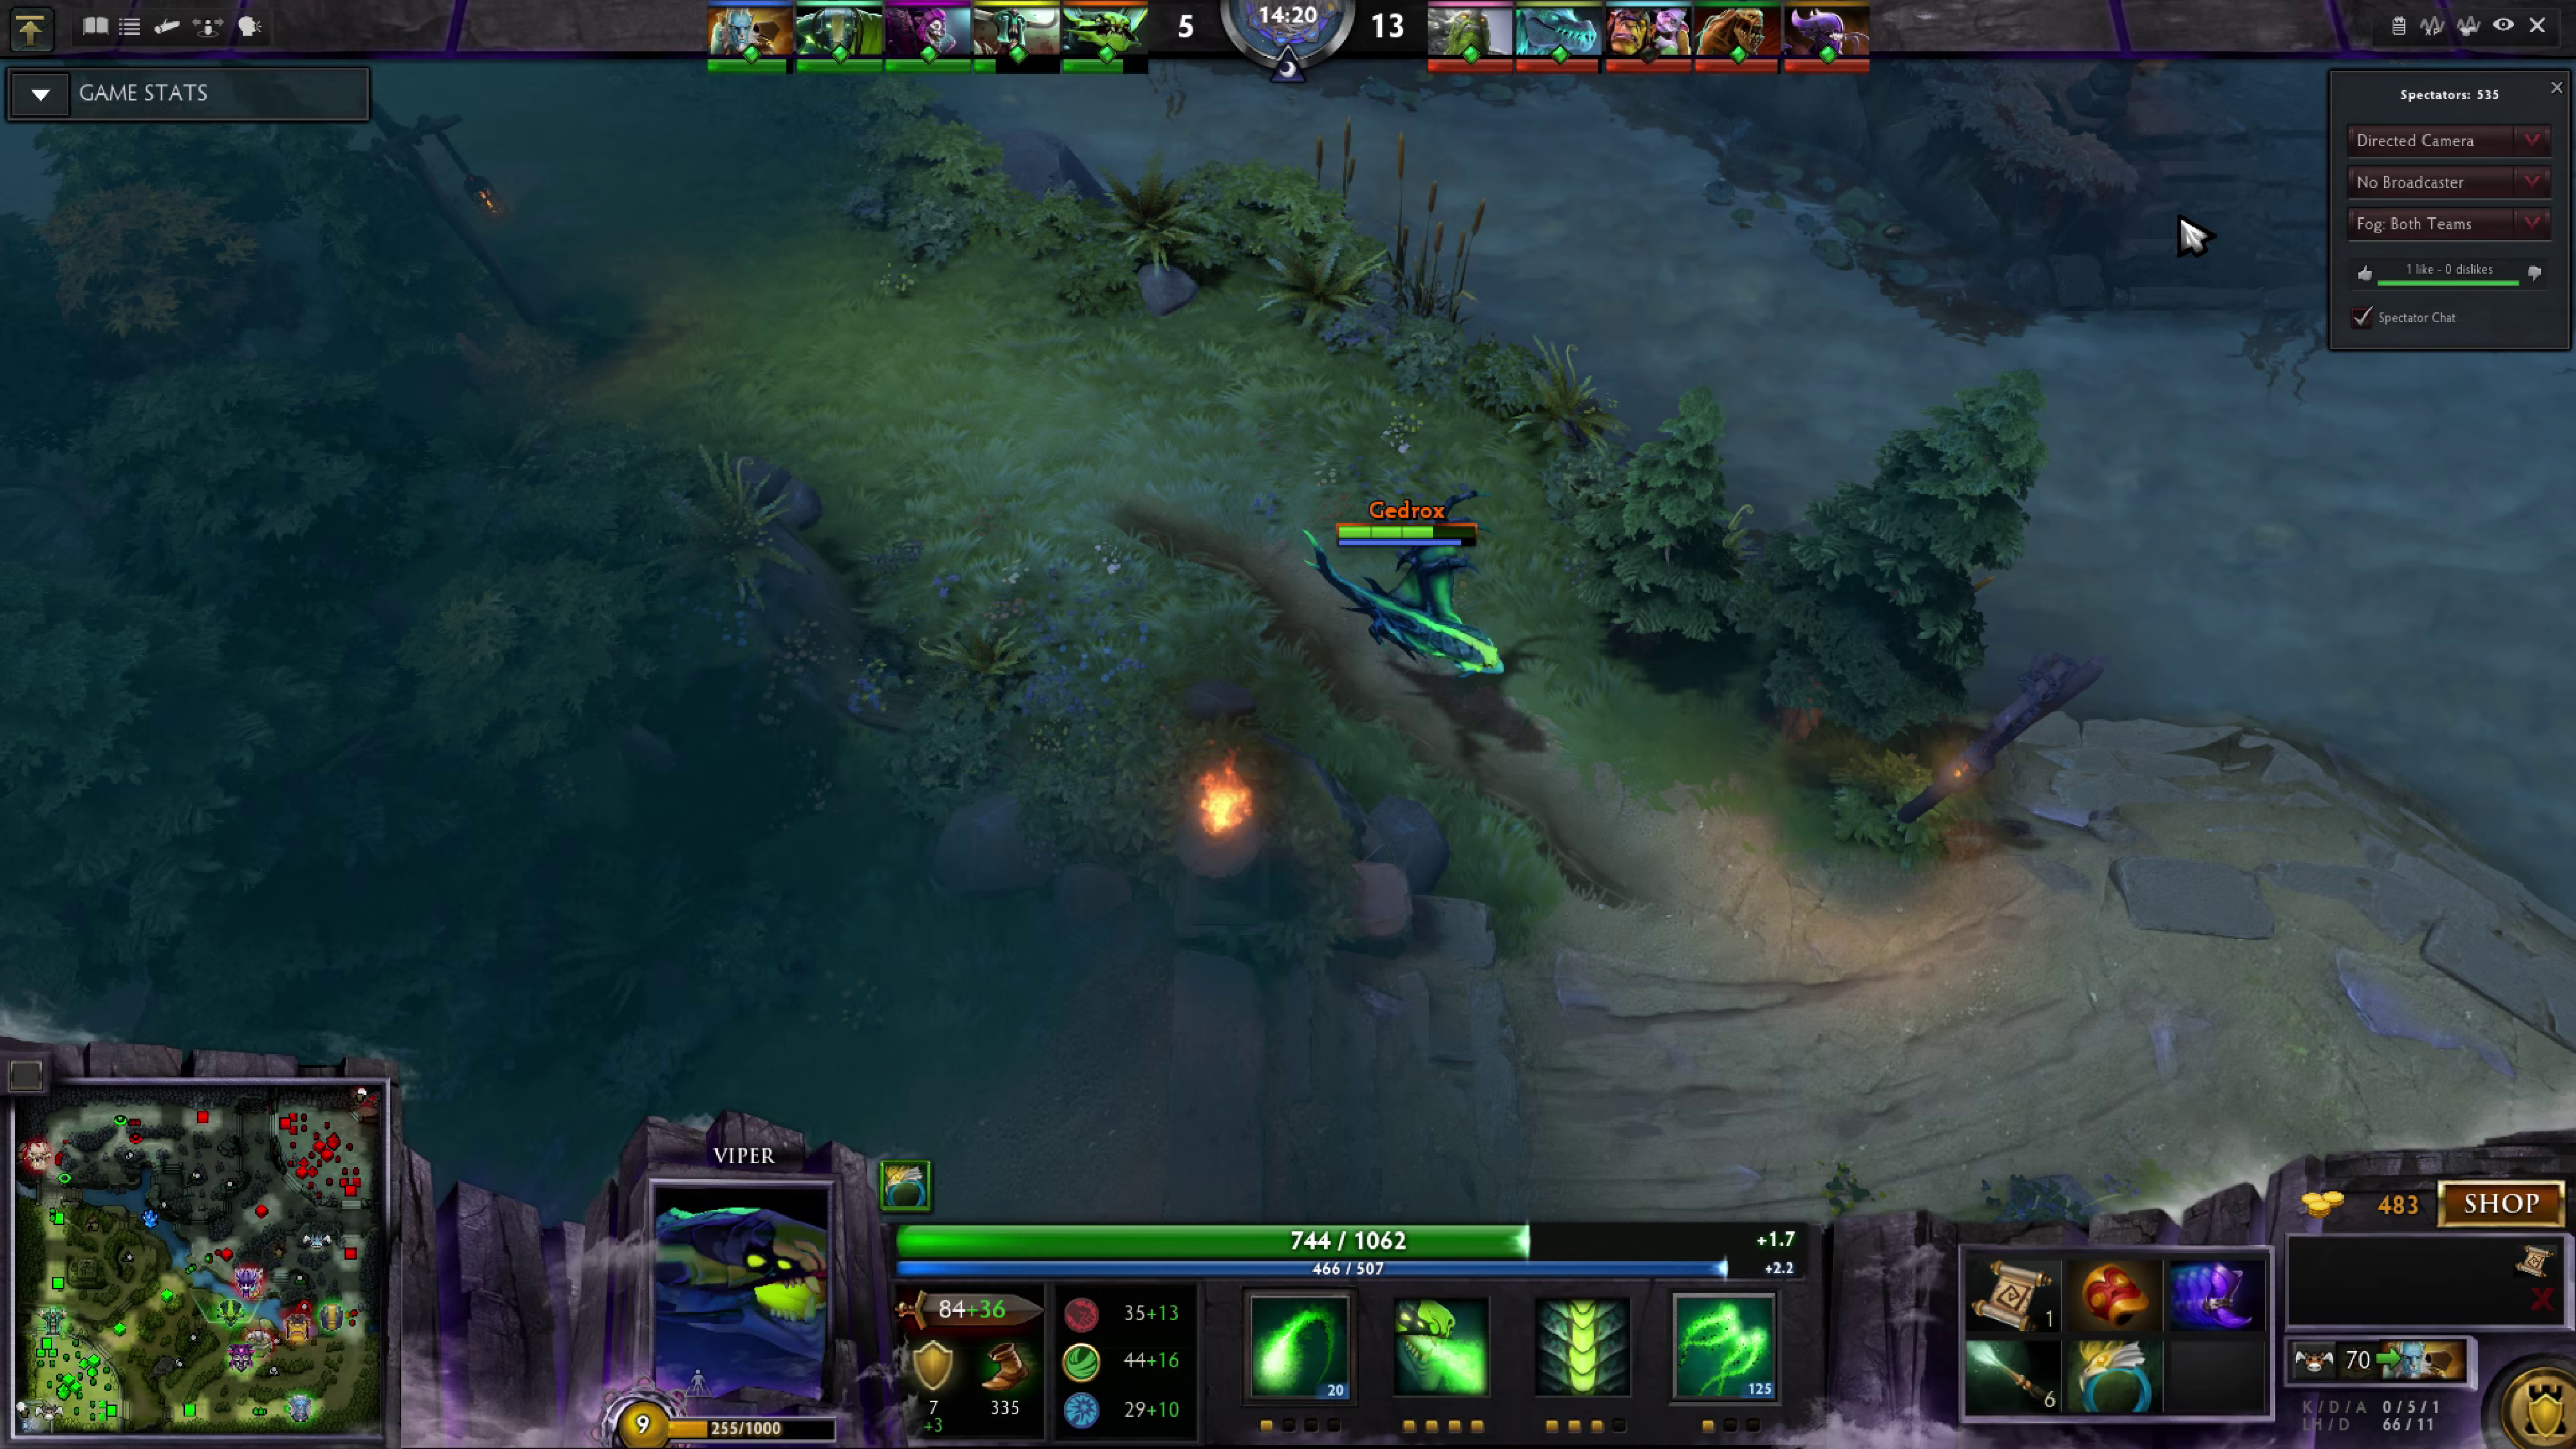
\includegraphics[width=0.885\textwidth]{dota2_jnd_decode.png}}
    \subcaptionbox{md-stage调整的JND优化快速算法解码图像\label{fig:dota2-md-dec}}
                    [\textwidth]{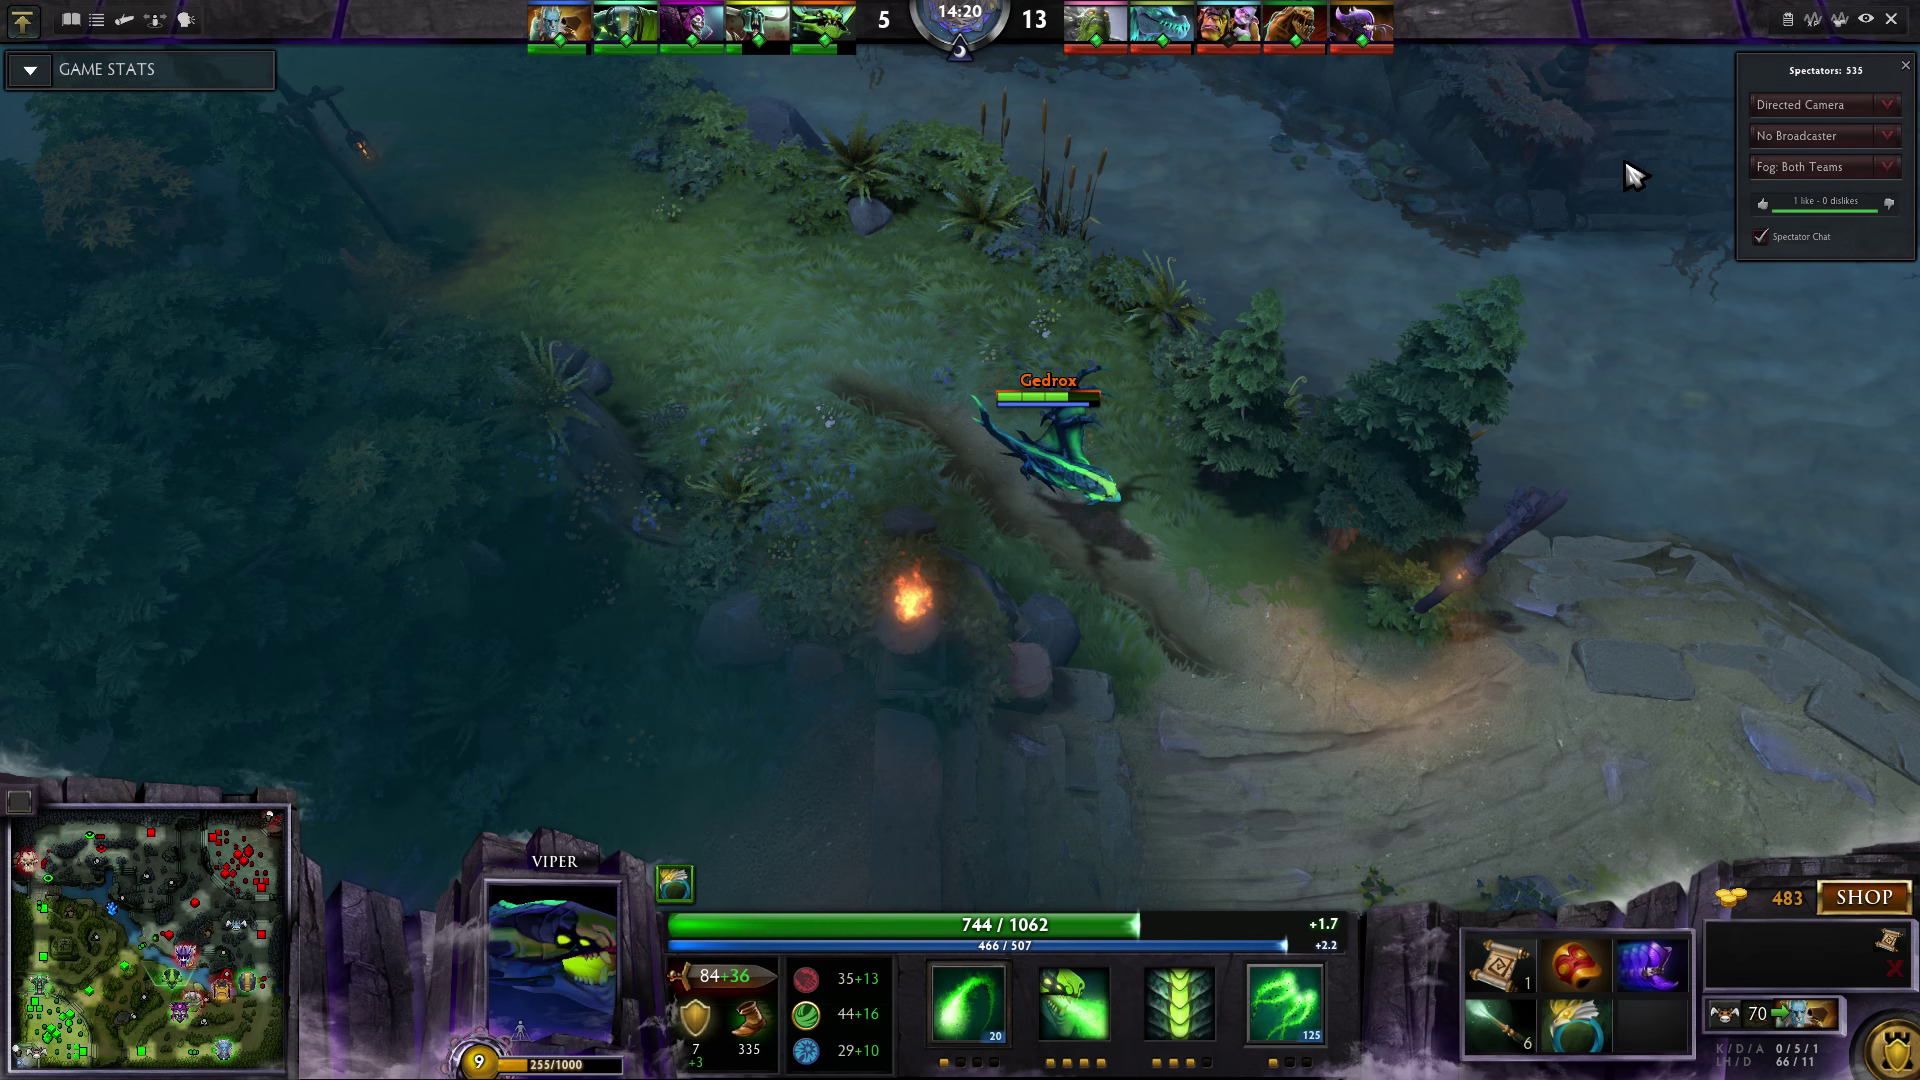
\includegraphics[width=0.885\textwidth]{dota2_md_dec.png}}
    \caption{原始算法与所提算法的解码对比图}
    \label{fig:dota2-decode}
  \end{figure}

  \section{本章小结}
  本章阐述了对于SVT-AV1编码器的低延迟优化工作。首先简要介绍了SVT-AV1编码器的架构、其系统资源管理器的原理、SVT架构中的三重并行与多阶段分区、模式选择决策。然后,介绍了对于SVT-AV1架构的编码延迟profile工具,该工具对后续的优化方向与测试结果起指导作用。另外,对于SVT-AV1还做了RESOURCE过程中的EOS优化,解决了EOS机制导致的1帧输入延迟;启用分tile优化时的竖向切分以降低编码延迟。

  本章还提出了基于JND的超级块快速划分算法。首先介绍了人眼视觉特性,包括亮度自适应性、视觉掩蔽效应和视觉注意机制,介绍了像素级JND模型的提出,以及根据像素级JND模型优化得到的块级JND模型。对JND感知阈值与AV1超级块划分结果进行统计分析,总结得到了与块划分相关的感知划分指标,并根据感知划分指标在twitch的游戏视频序列中的统计特性,分析确定了块划分提前终止划分的阈值。根据该阈值实现块划分时的提前终止,跳过了大量的搜索过程,减少大量编码复杂度,降低了编码时间。实验结果表明,在SVT-AV1的最快编码预设的基础上,在损失少量编码性能的前提下,本章所提出的超级块快速划分算法能够有效减少SVT-AV1的编码复杂度,从而降低SVT-AV1的编码延迟。